\subsection{Experimental Evaluation}
\label{sec:experiments}

Quantitative results are summarized in \tabref{tab:results-shapenet} (ShapeNet and KITTI) and \ref{tab:results-modelnet} (ModelNet). Qualitative results for the shape prior are shown in \figref{fig:results-shape-prior} and \ref{fig:results-latent-space}; shape completion results are shown in \figref{fig:results-synthetic} (ShapeNet and ModelNet) and \ref{fig:results-real} (KITTI and \Kinect).

\begin{figure}[t]
    \vspace*{-\figskipabove px}
    \centering
    \hspace*{-22px}
    \begin{subfigure}[t]{0.49\linewidth}
        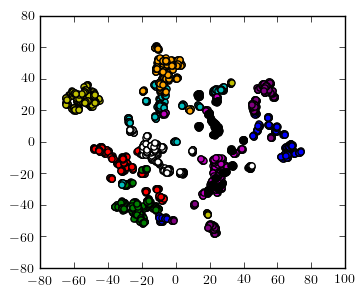
\includegraphics[height=3.1cm]{gls_modelnet10_codes_}
        \subcaption{\bf \DVAE t-SNE}
        \label{fig:results-latent-space-a1}
    \end{subfigure}
    \hspace*{-12px}
    \begin{subfigure}[t]{0.49\linewidth}
        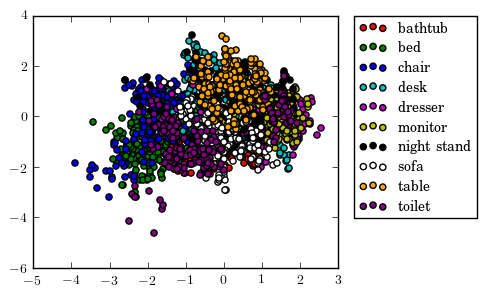
\includegraphics[height=3cm]{gls_modelnet10_codes2}
        \subcaption{\bf \DVAE Projection}
        \label{fig:results-latent-space-a2}
    \end{subfigure}
    \\
    \hspace*{-22px}
    \begin{subfigure}[t]{0.49\linewidth}
        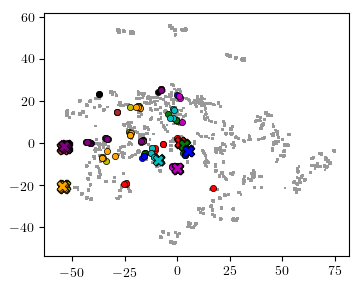
\includegraphics[height=3cm]{gls_clean_codes_outputs_}
        \subcaption{\bf \AML t-SNE}
        \label{fig:results-latent-space-b1}
    \end{subfigure}
    \hspace*{-12px}
    \begin{subfigure}[t]{0.49\linewidth}
        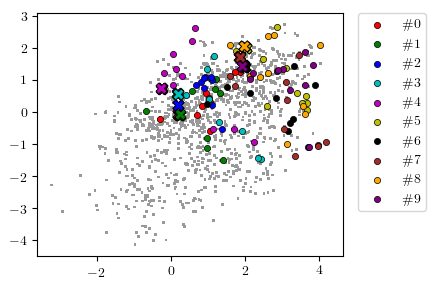
\includegraphics[height=3cm]{gls_clean_codes2_outputs}
        \subcaption{\bf \AML Projection}
        \label{fig:results-latent-space-b2}
    \end{subfigure}
    \vspace*{-\figskipcaption px}
    \caption{{\bf Learned Latent Spaces.} In (\subref{fig:results-latent-space-a1}) and (\subref{fig:results-latent-space-a2}), we show a t-SNE \citep{Maaten2008JMLR} visualization and a two-dimensional projection of the \DVAE latent space on ModelNet10. The plots illustrate that the \DVAE is able to separate the ten object categories. In (\subref{fig:results-latent-space-b1}) and (\subref{fig:results-latent-space-b2}), we show a t-SNE visualization and a projection of the latent space corresponding to our learned \AML model on \clean. We randomly picked $10$ ground truth shapes,  ``x'', and the corresponding observations ($10$ per shape), points (gray pixels indicate remaining shapes/observations). The plots illustrate that \AML is able to associate observations with the corresponding ground truth shapes under weak supervision.}
    \label{fig:results-latent-space}
    \vspace*{-\figskipbelow px}
\end{figure}
\begin{table*}[t]
    \vspace*{-\figskipabove px}
    \centering
    {\scriptsize
        \begin{tabularx}{1\textwidth}{|@{  }l@{  }|@{  }X@{  }|@{  }c@{  }c@{  }c@{  }c@{  }|@{  }c@{  }c@{  }c@{  }c@{  }|@{  }c@{  }|}
            \hline
             \multicolumn{1}{|@{  }c@{  }|@{  }}{Supervision} & \multicolumn{1}{@{  }c@{  }|@{  }}{Method} & \multicolumn{4}{@{  }c@{  }|@{  }}{\clean} & \multicolumn{4}{@{  }c@{  }|@{  }}{\noisy} & \multicolumn{1}{c|}{KITTI}\\
             \multicolumn{1}{|@{  }c@{  }|@{  }}{in \%} && \Abs {\tiny $\downarrow$} & \IoU {\tiny $\uparrow$} & \Acc [vx] {\tiny $\downarrow$} & \Compl [vx] {\tiny $\downarrow$} & \Abs {\tiny $\downarrow$} & \IoU {\tiny $\uparrow$} & \Acc [vx] {\tiny $\downarrow$} & \Compl [vx] {\tiny $\downarrow$} & \Compl [m] {\tiny $\downarrow$} \\
            \hline\hline
            \multicolumn{11}{|c|}{Low Resolution: $24 \times 54 \times 24$ voxels; * independent of resolution}\\
            \hline\hline
            {\color{darkgray}(shape prior)} & {\leavevmode\color{darkgray}\DVAE} & {\color{darkgray}0.019} & {\color{darkgray}0.885} & {\color{darkgray}0.283} & {\color{darkgray}0.527} & \multicolumn{5}{@{  }c@{  }|}{{\color{darkgray}(same shape prior as on \clean)}}\\
            \hline\hline
            \multirow{2}{*}{$\hphantom{<}100$} & \cite{Dai2017CVPRa} (\Dai) & {\bf\color{rred} 0.021} & {\bf\color{rred} 0.872} & {\bf\color{rred} 0.321} & {\bf\color{rred} 0.564} & {\bf\color{rred} 0.027} & {\bf\color{rred} 0.836} & {\bf\color{rred} 0.391} & {\bf\color{rred} 0.633} & 0.128\\
            &\Sup & 0.026 & 0.841 & 0.409 & 0.607 & 0.028 & 0.833 & 0.407 & 0.637 & {\bf\color{rred} 0.091}\\
            \hline
            \multirow{10}{*}{$<7.7$} &\BL & 0.067 & 0.596 & 0.999 & 1.335 & 0.064 & 0.609 & 0.941 & 1.29 & \color{darkgray}--\\
            &\M & 0.052 & 0.697 & 0.79 & 0.938 & 0.052 & 0.696 & 0.79 & 0.938 & \color{darkgray}--\\
            &\ML & 0.04 & 0.756 & 0.637 & 0.8 & 0.041 & 0.755 & 0.625 & 0.829 & \color{darkgray}(too slow)\\
            & *\cite{Gupta2015CVPR} (\ICP) & \multicolumn{2}{@{  }c@{  }}{\color{darkgray}(mesh only)} & 0.534 & {\bf\color{rgreen} 0.503} & \multicolumn{2}{@{  }c@{  }}{\color{darkgray}(mesh only)} & 7.551 & 6.372 & \color{darkgray}(too slow)\\
            & *\cite{Engelmann2016GCPR} (\Engelmann) & \multicolumn{2}{@{  }c@{  }}{\color{darkgray}(mesh only)} & 1.235 & 1.237 & \multicolumn{2}{@{  }c@{  }}{\color{darkgray}(mesh only)} & 1.974 & 1.312 & 0.13\\ % 0.545016
            &\dAML & {\bf\color{rgreen} 0.034} & {\bf\color{rgreen} 0.784} & {\bf\color{rgreen} 0.532} & 0.741 & {\bf\color{rgreen} 0.036} & {\bf\color{rgreen} 0.772} & {\bf\color{rgreen} 0.557} & {\bf\color{rgreen} 0.76} & \color{darkgray}(see \AML)\\
            &\AML & {\bf\color{rgreen} 0.034} & 0.779 & 0.549 & 0.753 & {\bf\color{rgreen} 0.036} & 0.771 & 0.57 & 0.761 & {\bf\color{rgreen} 0.12}\\
            \hline\hline
            \multicolumn{11}{|c|}{Low Resolution: $24 \times 54 \times 24$ voxels; Multiple, $k > 1$ Fused Views}\\
            \hline\hline
            \multirow{2}{*}{$\hphantom{<}100$} & \cite{Dai2017CVPRa} (\Dai), $k = 5$ & \bf\color{rred}0.012 & \bf\color{rred}0.924 & \bf\color{rred}0.214 & \bf\color{rred}0.436 & \bf\color{rred}0.018 & \bf\color{rred}0.887 & \bf\color{rred}0.278 & \bf\color{rred}0.491 &\multirow{2}{*}{\color{darkgray}n/a}\\
            &\Sup, $k = 5$ & 0.022 & 0.866 & 0.336 & 0.566 & 0.024 & 0.86 & 0.331 & 0.573 &\\
            \hline
            $<16$ & \AML, $k = 2$ & 0.032 & 0.794 & 0.489 & 0.695 & 0.034 & 0.79 & 0.52 & 0.725 & \multirow{3}{*}{\color{darkgray}n/a}\\
            $<24$ & \AML, $k = 3$ & {\bf\color{rgreen} 0.031} & {\bf\color{rgreen} 0.809} & {\bf\color{rgreen} 0.471} & {\bf\color{rgreen} 0.667} & {\bf\color{rgreen} 0.031} & {\bf\color{rgreen} 0.81} & {\bf\color{rgreen} 0.493} & {\bf\color{rgreen} 0.67} &\\
            $<40$ & \AML, $k = 5$ & {\bf\color{rgreen} 0.031} & 0.804 & 0.502 & 0.686 & 0.035 & 0.799 & 0.523 & 0.7 &\\
            \hline\hline
            \multicolumn{11}{|c|}{Medium Resolution: $32 \times 72 \times 32$ voxels}\\
            \hline\hline
            {\color{darkgray}(shape prior)} & {\leavevmode\color{darkgray}\DVAE} & {\color{darkgray}0.019} & {\color{darkgray}0.877} & {\color{darkgray}0.24} & {\color{darkgray}0.47} & \multicolumn{5}{@{  }c@{  }|}{{\color{darkgray}(same shape prior as on \clean)}}\\
            \hline\hline 
            \multirow{2}{*}{$\hphantom{<}100$} & \cite{Dai2017CVPRa} (\Dai) & {\bf\color{rred} 0.02} & {\bf\color{rred} 0.869} & {\bf\color{rred} 0.399} & {\bf\color{rred} 0.674} & {\bf\color{rred} 0.026} & {\bf\color{rred} 0.83} & {\bf\color{rred} 0.51} & {\bf\color{rred} 0.767} & {\bf\color{rred} 0.074}\\
            &\Sup & 0.027 & 0.834 & 0.498 & 0.789 & 0.029 & 0.815 & 0.571 & 0.843 & 0.09\\
            \hline
            $\leq6.1$ & \AML & {\bf\color{rgreen} 0.031} & {\bf\color{rgreen} 0.788} & {\bf\color{rgreen} 0.415} & {\bf\color{rgreen} 0.584} & {\bf\color{rgreen} 0.036} & {\bf\color{rgreen} 0.766} & {\bf\color{rgreen} 0.721} & {\bf\color{rgreen} 0.953} & {\bf\color{rgreen} 0.083}\\
            \hline\hline
            \multicolumn{11}{|c|}{High Resolution: $48 \times 108 \times 48$ voxels}\\
            \hline\hline
            {\color{darkgray}(shape prior)} & {\leavevmode\color{darkgray}\DVAE} & {\color{darkgray}0.018} & \color{darkgray}0.87 & {\color{darkgray}0.272} & {\color{darkgray}0.434} & \multicolumn{5}{@{  }c@{  }|}{{\color{darkgray}(same shape prior as on \clean)}}\\
            \hline\hline
            \multirow{2}{*}{$\hphantom{<}100$} & \Dai & {\bf\color{rred} 0.017} & {\bf\color{rred} 0.88} & {\bf\color{rred} 0.517} & {\bf\color{rred} 0.827} & 0.054 & 0.664 & 1.559 & 2.067 & {\bf\color{rred} 0.066}\\
            &\Sup & 0.023 & 0.843 & 0.677 & 1.032 & {\bf\color{rred} 0.052} & {\bf\color{rred} 0.674} & {\bf\color{rred} 1.52} & {\bf\color{rred} 1.981} & 0.091\\
            \hline
            $<3.5$ & \AML & {\bf\color{rgreen} 0.028} & {\bf\color{rgreen} 0.796} & {\bf\color{rgreen} 0.433} & {\bf\color{rgreen} 0.579} & {\bf\color{rgreen} 0.045} & {\bf\color{rgreen} 0.659} & {\bf\color{rgreen} 1.4} & {\bf\color{rgreen} 1.957} & {\bf\color{rgreen} 0.078}\\
            \hline
        \end{tabularx}
    }
    \vspace*{-\figskipcaption px}
    \caption{{\bf Quantitative Results on ShapeNet and KITTI.} We consider Hamming distance (\Abs) and intersection over union (\IoU) for occupancy grids as well as accuracy (\Acc) and completeness (\Compl) for meshes on \clean, \noisy and KITTI. For \Abs, \Acc and \Compl, lower is better; for \IoU, higher is better. The unit of \Acc and \Compl is voxels (voxel length at $24 \ntimes 54 \ntimes 48$ voxels) or meters. Note that the \DVAE shape prior (in {\color{darkgray}gray}) is only reported as reference (\ie, bound on (d)\AML). We indicate the level of supervision in percentage, relative to the corresponding resolution and mark the best results under full supervision in {\color{rred}\bf red} and under weak supervision in {\color{rgreen}\bf green}.}
    \label{tab:results-shapenet}
    \vspace*{-\figskipbelow px}
\end{table*}
\newcommand{\cleana}{231} % 165 alternative
\newcommand{\cleanb}{297}

\newcommand{\noisya}{132}
\newcommand{\noisyb}{66}

\newcommand{\bathtuba}{792}
\newcommand{\bathtubb}{330}

\newcommand{\chaira}{528}
\newcommand{\chairb}{990} % 0 924

\newcommand{\deska}{264} % 198
\newcommand{\deskb}{858}

\newcommand{\tablea}{858}
\newcommand{\tableb}{396} % 600 594
\begin{figure*}[t]
    \vspace*{-\figskipabove px}
    \vspace*{2px}
    \centering
    {\scriptsize
    \begin{subfigure}[t]{1\textwidth}
        \begin{subfigure}[t]{0.095\textwidth}
        	\vspace{0px}\centering
        	Obs\\
        	\includegraphics[width=1.8cm,trim={\cropleft cm \croplower cm \cropright cm \cropupper cm},clip]{gdat_shapenet_clean_low_\cleana_points}
        \end{subfigure}
        \begin{subfigure}[t]{0.095\textwidth}
        	\vspace{0px}\centering
        	\Dai\\
        	\includegraphics[width=1.8cm,trim={\cropleft cm \croplower cm \cropright cm \cropupper cm},clip]{gexp_clean_low_10_wide_sup_3_2_res_\cleana}
        \end{subfigure}
        \begin{subfigure}[t]{0.095\textwidth}
            \vspace{0px}\centering
            \Dai\\
            \includegraphics[width=1.8cm,trim={\cropleft cm \croplower cm \cropright cm \cropupper cm},clip]{gexp_clean_low_10_wide_sup_3_3_res_\cleana}
        \end{subfigure}
        \begin{subfigure}[t]{0.095\textwidth}
            \vspace{0px}\centering
            \Engelmann\\
            \includegraphics[width=1.8cm,trim={\cropleft cm \croplower cm \cropright cm \cropupper cm},clip]{gexp_clean_low_10_wide_rw_results_\cleana}
        \end{subfigure}
        \begin{subfigure}[t]{0.095\textwidth}
            \vspace{0px}\centering
            \ML\\
            \includegraphics[width=1.8cm,trim={\cropleft cm \croplower cm \cropright cm \cropupper cm},clip]{gexp_clean_low_10_wide_ml_3_2_res_\cleana}
        \end{subfigure}
        \begin{subfigure}[t]{0.095\textwidth}
            \vspace{0px}\centering
            \ML\\
            \includegraphics[width=1.8cm,trim={\cropleft cm \croplower cm \cropright cm \cropupper cm},clip]{gexp_clean_low_10_wide_ml_3_3_res_\cleana}
        \end{subfigure}
        \begin{subfigure}[t]{0.095\textwidth}
        	\vspace{0px}\centering
        	\AML\\
        	\includegraphics[width=1.8cm,trim={\cropleft cm \croplower cm \cropright cm \cropupper cm},clip]{gexp_clean_low_10_wide_vae_aml_3_2_res_\cleana}
        \end{subfigure}
        \begin{subfigure}[t]{0.095\textwidth}
            \vspace{0px}\centering
            \AML\\
            \includegraphics[width=1.8cm,trim={\cropleft cm \croplower cm \cropright cm \cropupper cm},clip]{gexp_clean_low_10_wide_vae_aml_3_3_res_\cleana}
        \end{subfigure}
        \begin{subfigure}[t]{0.095\textwidth}
        	\vspace{0px}\centering
        	GT\\
        	\includegraphics[width=1.8cm,trim={\cropleft cm \croplower cm \cropright cm \cropupper cm},clip]{gdat_shapenet_clean_low_\cleana_gt}
        \end{subfigure}
        \begin{subfigure}[t]{0.095\textwidth}
            \vspace{0px}\centering
            GT\\
            \includegraphics[width=1.8cm,trim={\cropleft cm \croplower cm \cropright cm \cropupper cm},clip]{gdat_shapenet_clean_low_\cleana_bin}
        \end{subfigure}
        \\[-2px]
        \begin{subfigure}[t]{0.095\textwidth}
        	\vspace{0px}\centering
        	%Obs\\
        	\includegraphics[width=1.8cm,trim={\cropleft cm \croplower cm \cropright cm \cropupper cm},clip]{gdat_shapenet_clean_low_\cleanb_points}
        \end{subfigure}
        \begin{subfigure}[t]{0.095\textwidth}
        	\vspace{0px}\centering
        	%\Dai\\
        	\includegraphics[width=1.8cm,trim={\cropleft cm \croplower cm \cropright cm \cropupper cm},clip]{gexp_clean_low_10_wide_sup_3_2_res_\cleanb}
        \end{subfigure}
        \begin{subfigure}[t]{0.095\textwidth}
        	\vspace{0px}\centering
        	%\Dai\\
        	\includegraphics[width=1.8cm,trim={\cropleft cm \croplower cm \cropright cm \cropupper cm},clip]{gexp_clean_low_10_wide_sup_3_3_res_\cleanb}
        \end{subfigure}
        \begin{subfigure}[t]{0.095\textwidth}
        	\vspace{0px}\centering
        	%\Engelmann\\
        	\includegraphics[width=1.8cm,trim={\cropleft cm \croplower cm \cropright cm \cropupper cm},clip]{gexp_clean_low_10_wide_rw_results_\cleanb}
        \end{subfigure}
        \begin{subfigure}[t]{0.095\textwidth}
            \vspace{0px}\centering
            %\ML\\
            \includegraphics[width=1.8cm,trim={\cropleft cm \croplower cm \cropright cm \cropupper cm},clip]{gexp_clean_low_10_wide_ml_3_2_res_\cleanb}
        \end{subfigure}
        \begin{subfigure}[t]{0.095\textwidth}
        	\vspace{0px}\centering
        	%\ML\\
        	\includegraphics[width=1.8cm,trim={\cropleft cm \croplower cm \cropright cm \cropupper cm},clip]{gexp_clean_low_10_wide_ml_3_3_res_\cleanb}
        \end{subfigure}
        \begin{subfigure}[t]{0.095\textwidth}
        	\vspace{0px}\centering
        	%\AML\\
        	\includegraphics[width=1.8cm,trim={\cropleft cm \croplower cm \cropright cm \cropupper cm},clip]{gexp_clean_low_10_wide_vae_aml_3_2_res_\cleanb}
        \end{subfigure}
        \begin{subfigure}[t]{0.095\textwidth}
        	\vspace{0px}\centering
        	%\AML\\
        	\includegraphics[width=1.8cm,trim={\cropleft cm \croplower cm \cropright cm \cropupper cm},clip]{gexp_clean_low_10_wide_vae_aml_3_3_res_\cleanb}
        \end{subfigure}
        \begin{subfigure}[t]{0.095\textwidth}
        	\vspace{0px}\centering
        	%GT\\
        	\includegraphics[width=1.8cm,trim={\cropleft cm \croplower cm \cropright cm \cropupper cm},clip]{gdat_shapenet_clean_low_\cleanb_gt}
        \end{subfigure}
        \begin{subfigure}[t]{0.095\textwidth}
        	\vspace{0px}\centering
        	%GT\\
        	\includegraphics[width=1.8cm,trim={\cropleft cm \croplower cm \cropright cm \cropupper cm},clip]{gdat_shapenet_clean_low_\cleanb_bin}
        \end{subfigure}
        \begin{subfigure}[t]{0.095\textwidth}
        	\vspace{0px}\centering
        	%Obs\\
        	\includegraphics[width=1.8cm,trim={\cropleft cm \croplower cm \cropright cm \cropupper cm},clip]{gdat_shapenet_noisy_low_\noisya_points}
        \end{subfigure}
        \begin{subfigure}[t]{0.095\textwidth}
        	\vspace{0px}\centering
        	%\Dai\\
        	\includegraphics[width=1.8cm,trim={\cropleft cm \croplower cm \cropright cm \cropupper cm},clip]{gexp_noisy_low_10_wide_w2_1_sup_3_2_res_\noisya}
        \end{subfigure}
        \begin{subfigure}[t]{0.095\textwidth}
            \vspace{0px}\centering
            %\Dai\\
            \includegraphics[width=1.8cm,trim={\cropleft cm \croplower cm \cropright cm \cropupper cm},clip]{gexp_noisy_low_10_wide_w2_1_sup_3_3_res_\noisya}
        \end{subfigure}
        \begin{subfigure}[t]{0.095\textwidth}
        	\vspace{0px}\centering
        	%\Engelmann\\
        	\includegraphics[width=1.8cm,trim={\cropleft cm \croplower cm \cropright cm \cropupper cm},clip]{gexp_noisy_low_10_wide_w2_1_rw_results_\noisya}
        \end{subfigure}
        \begin{subfigure}[t]{0.095\textwidth}
            \vspace{0px}\centering
            %\ML\\
            \includegraphics[width=1.8cm,trim={\cropleft cm \croplower cm \cropright cm \cropupper cm},clip]{gexp_noisy_low_10_wide_w2_1_ml_3_2_res_\noisya}
        \end{subfigure}
        \begin{subfigure}[t]{0.095\textwidth}
            \vspace{0px}\centering
            %\ML\\
            \includegraphics[width=1.8cm,trim={\cropleft cm \croplower cm \cropright cm \cropupper cm},clip]{gexp_noisy_low_10_wide_w2_1_ml_3_3_res_\noisya}
        \end{subfigure}
        \begin{subfigure}[t]{0.095\textwidth}
        	\vspace{0px}\centering
        	%\AML\\
        	\includegraphics[width=1.8cm,trim={\cropleft cm \croplower cm \cropright cm \cropupper cm},clip]{gexp_noisy_low_10_wide_w2_1_vae_aml_3_2_res_\noisya}
        \end{subfigure}
        \begin{subfigure}[t]{0.095\textwidth}
        	\vspace{0px}\centering
        	%\AML\\
        	\includegraphics[width=1.8cm,trim={\cropleft cm \croplower cm \cropright cm \cropupper cm},clip]{gexp_noisy_low_10_wide_w2_1_vae_aml_3_3_res_\noisya}
        \end{subfigure}
        \begin{subfigure}[t]{0.095\textwidth}
        	\vspace{0px}\centering
        	%GT\\
        	\includegraphics[width=1.8cm,trim={\cropleft cm \croplower cm \cropright cm \cropupper cm},clip]{gdat_shapenet_noisy_low_\noisya_gt}
        \end{subfigure}
        \begin{subfigure}[t]{0.095\textwidth}
            \vspace{0px}\centering
            %GT\\
            \includegraphics[width=1.8cm,trim={\cropleft cm \croplower cm \cropright cm \cropupper cm},clip]{gdat_shapenet_noisy_low_\noisya_bin}
        \end{subfigure}
        \\[-2px]
        \begin{subfigure}[t]{0.095\textwidth}
        	\vspace{0px}\centering
        	%Obs\\
        	\includegraphics[width=1.8cm,trim={\cropleft cm \croplower cm \cropright cm \cropupper cm},clip]{gdat_shapenet_noisy_low_\noisyb_points}
        \end{subfigure}
        \begin{subfigure}[t]{0.095\textwidth}
        	\vspace{0px}\centering
        	%\Dai\\
        	\includegraphics[width=1.8cm,trim={\cropleft cm \croplower cm \cropright cm \cropupper cm},clip]{gexp_noisy_low_10_wide_w2_1_sup_3_2_res_\noisyb}
        \end{subfigure}
        \begin{subfigure}[t]{0.095\textwidth}
        	\vspace{0px}\centering
        	%\Dai\\
        	\includegraphics[width=1.8cm,trim={\cropleft cm \croplower cm \cropright cm \cropupper cm},clip]{gexp_noisy_low_10_wide_w2_1_sup_3_3_res_\noisyb}
        \end{subfigure}
        \begin{subfigure}[t]{0.095\textwidth}
        	\vspace{0px}\centering
        	%\Engelmann\\
        	\includegraphics[width=1.8cm,trim={\cropleft cm \croplower cm \cropright cm \cropupper cm},clip]{gexp_noisy_low_10_wide_w2_1_rw_results_\noisyb}
        \end{subfigure}
        \begin{subfigure}[t]{0.095\textwidth}
            \vspace{0px}\centering
            %\ML\\
            \includegraphics[width=1.8cm,trim={\cropleft cm \croplower cm \cropright cm \cropupper cm},clip]{gexp_noisy_low_10_wide_w2_1_ml_3_2_res_\noisyb}
        \end{subfigure}
        \begin{subfigure}[t]{0.095\textwidth}
        	\vspace{0px}\centering
        	%\ML\\
        	\includegraphics[width=1.8cm,trim={\cropleft cm \croplower cm \cropright cm \cropupper cm},clip]{gexp_noisy_low_10_wide_w2_1_ml_3_3_res_\noisyb}
        \end{subfigure}
        \begin{subfigure}[t]{0.095\textwidth}
        	\vspace{0px}\centering
        	%\AML\\
        	\includegraphics[width=1.8cm,trim={\cropleft cm \croplower cm \cropright cm \cropupper cm},clip]{gexp_noisy_low_10_wide_w2_1_vae_aml_3_2_res_\noisyb}
        \end{subfigure}
        \begin{subfigure}[t]{0.095\textwidth}
        	\vspace{0px}\centering
        	%\AML\\
        	\includegraphics[width=1.8cm,trim={\cropleft cm \croplower cm \cropright cm \cropupper cm},clip]{gexp_noisy_low_10_wide_w2_1_vae_aml_3_3_res_\noisyb}
        \end{subfigure}
        \begin{subfigure}[t]{0.095\textwidth}
        	\vspace{0px}\centering
        	%GT\\
        	\includegraphics[width=1.8cm,trim={\cropleft cm \croplower cm \cropright cm \cropupper cm},clip]{gdat_shapenet_noisy_low_\noisyb_gt}
        \end{subfigure}
        \begin{subfigure}[t]{0.095\textwidth}
        	\vspace{0px}\centering
        	%GT\\
        	\includegraphics[width=1.8cm,trim={\cropleft cm \croplower cm \cropright cm \cropupper cm},clip]{gdat_shapenet_noisy_low_\noisyb_bin}
        \end{subfigure}
        \subcaption{\clean (Top) and \noisy (Bottom), Low Resolution ($24\ntimes54\ntimes24$)}
    \end{subfigure}
    \\[4px]
    \begin{subfigure}[t]{1\textwidth}
   		\begin{subfigure}[t]{0.095\textwidth}
   			\vspace{0px}\centering
   			Obs\\
   			\includegraphics[width=1.8cm,trim={\cropleft cm \croplower cm \cropright cm \cropupper cm},clip]{gdat_modelnet_bathtub_low_\bathtuba_points}
   		\end{subfigure}
   		\begin{subfigure}[t]{0.095\textwidth}
   			\vspace{0px}\centering
   			\Dai\\
   			\includegraphics[width=1.8cm,trim={\cropleft cm \croplower cm \cropright cm \cropupper cm},clip]{gexp_clean_bathtub_low_10_wide_sup_3_2_res_\bathtuba}
   		\end{subfigure}
   		\begin{subfigure}[t]{0.095\textwidth}
   			\vspace{0px}\centering
   			\Dai\\
   			\includegraphics[width=1.8cm,trim={\cropleft cm \croplower cm \cropright cm \cropupper cm},clip]{gexp_clean_bathtub_low_10_wide_sup_3_3_res_\bathtuba}
   		\end{subfigure}
   		\begin{subfigure}[t]{0.095\textwidth}
   			\vspace{0px}\centering
   			\ICP\\
   			\includegraphics[width=1.8cm,trim={\cropleft cm \croplower cm \cropright cm \cropupper cm},clip]{gexp_clean_bathtub_low_10_wide_icp_3_2_res_\bathtuba}
   		\end{subfigure}
        \begin{subfigure}[t]{0.095\textwidth}
            \vspace{0px}\centering
            \ML\\
            \includegraphics[width=1.8cm,trim={\cropleft cm \croplower cm \cropright cm \cropupper cm},clip]{gexp_clean_bathtub_low_10_wide_ml_3_2_res_\bathtuba}
        \end{subfigure}
   		\begin{subfigure}[t]{0.095\textwidth}
   			\vspace{0px}\centering
   			\ML\\
   			\includegraphics[width=1.8cm,trim={\cropleft cm \croplower cm \cropright cm \cropupper cm},clip]{gexp_clean_bathtub_low_10_wide_ml_3_3_res_\bathtuba}
   		\end{subfigure}
   		\begin{subfigure}[t]{0.095\textwidth}
   			\vspace{0px}\centering
   			\AML\\
   			\includegraphics[width=1.8cm,trim={\cropleft cm \croplower cm \cropright cm \cropupper cm},clip]{gexp_clean_bathtub_low_10_wide_vae_aml_3_2_res_\bathtuba}
   		\end{subfigure}
   		\begin{subfigure}[t]{0.095\textwidth}
   			\vspace{0px}\centering
   			\AML\\
   			\includegraphics[width=1.8cm,trim={\cropleft cm \croplower cm \cropright cm \cropupper cm},clip]{gexp_clean_bathtub_low_10_wide_vae_aml_3_3_res_\bathtuba}
   		\end{subfigure}
   		\begin{subfigure}[t]{0.095\textwidth}
   			\vspace{0px}\centering
   			GT\\
   			\includegraphics[width=1.8cm,trim={\cropleft cm \croplower cm \cropright cm \cropupper cm},clip]{gdat_modelnet_bathtub_low_\bathtuba_gt}
   		\end{subfigure}
   		\begin{subfigure}[t]{0.095\textwidth}
   			\vspace{0px}\centering
   			GT\\
   			\includegraphics[width=1.8cm,trim={\cropleft cm \croplower cm \cropright cm \cropupper cm},clip]{gdat_modelnet_bathtub_low_\bathtuba_bin}
   		\end{subfigure}
   		\\[2px]
   		\begin{subfigure}[t]{0.095\textwidth}
   			\vspace{0px}\centering
   			%Obs\\
   			\includegraphics[width=1.8cm,trim={\cropleft cm \croplower cm \cropright cm \cropupper cm},clip]{gdat_modelnet_chair_low_\chaira_points}
   		\end{subfigure}
   		\begin{subfigure}[t]{0.095\textwidth}
   			\vspace{0px}\centering
   			%\Dai\\
   			\includegraphics[width=1.8cm,trim={\cropleft cm \croplower cm \cropright cm \cropupper cm},clip]{gexp_clean_chair_low_10_wide_sup_3_2_res_\chaira}
   		\end{subfigure}
   		\begin{subfigure}[t]{0.095\textwidth}
   			\vspace{0px}\centering
   			%\Dai\\
   			\includegraphics[width=1.8cm,trim={\cropleft cm \croplower cm \cropright cm \cropupper cm},clip]{gexp_clean_chair_low_10_wide_sup_3_3_res_\chaira}
   		\end{subfigure}
   		\begin{subfigure}[t]{0.095\textwidth}
   			\vspace{0px}\centering
   			%\ICP\\
   			\includegraphics[width=1.8cm,trim={\cropleft cm \croplower cm \cropright cm \cropupper cm},clip]{gexp_clean_chair_low_10_wide_icp_3_2_res_\chaira}
   		\end{subfigure}
        \begin{subfigure}[t]{0.095\textwidth}
            \vspace{0px}\centering
            %\ML\\
            \includegraphics[width=1.8cm,trim={\cropleft cm \croplower cm \cropright cm \cropupper cm},clip]{gexp_clean_chair_low_10_wide_ml_3_2_res_\chaira}
        \end{subfigure}
   		\begin{subfigure}[t]{0.095\textwidth}
   			\vspace{0px}\centering
   			%\ML\\
   			\includegraphics[width=1.8cm,trim={\cropleft cm \croplower cm \cropright cm \cropupper cm},clip]{gexp_clean_chair_low_10_wide_ml_3_3_res_\chaira}
   		\end{subfigure}
   		\begin{subfigure}[t]{0.095\textwidth}
   			\vspace{0px}\centering
   			%\AML\\
   			\includegraphics[width=1.8cm,trim={\cropleft cm \croplower cm \cropright cm \cropupper cm},clip]{gexp_clean_chair_low_10_wide_vae_aml_3_2_res_\chaira}
   		\end{subfigure}
   		\begin{subfigure}[t]{0.095\textwidth}
   			\vspace{0px}\centering
   			%\AML\\
   			\includegraphics[width=1.8cm,trim={\cropleft cm \croplower cm \cropright cm \cropupper cm},clip]{gexp_clean_chair_low_10_wide_vae_aml_3_3_res_\chaira}
   		\end{subfigure}
   		\begin{subfigure}[t]{0.095\textwidth}
   			\vspace{0px}\centering
   			%GT\\
   			\includegraphics[width=1.8cm,trim={\cropleft cm \croplower cm \cropright cm \cropupper cm},clip]{gdat_modelnet_chair_low_\chaira_gt}
   		\end{subfigure}
   		\begin{subfigure}[t]{0.095\textwidth}
   			\vspace{0px}\centering
   			%GT\\
   			\includegraphics[width=1.8cm,trim={\cropleft cm \croplower cm \cropright cm \cropupper cm},clip]{gdat_modelnet_chair_low_\chaira_bin}
   		\end{subfigure}
   		\\[2px]
   		\begin{subfigure}[t]{0.095\textwidth}
   			\vspace{0px}\centering
   			%Obs\\
   			\includegraphics[width=1.8cm,trim={\cropleft cm \croplower cm \cropright cm \cropupper cm},clip]{gdat_modelnet_desk_low_\deska_points}
   		\end{subfigure}
   		\begin{subfigure}[t]{0.095\textwidth}
   			\vspace{0px}\centering
   			%\Dai\\
   			\includegraphics[width=1.8cm,trim={\cropleft cm \croplower cm \cropright cm \cropupper cm},clip]{gexp_clean_desk_low_10_wide_sup_3_2_res_\deska}
   		\end{subfigure}
   		\begin{subfigure}[t]{0.095\textwidth}
   			\vspace{0px}\centering
   			%\Dai\\
   			\includegraphics[width=1.8cm,trim={\cropleft cm \croplower cm \cropright cm \cropupper cm},clip]{gexp_clean_desk_low_10_wide_sup_3_3_res_\deska}
   		\end{subfigure}
   		\begin{subfigure}[t]{0.095\textwidth}
   			\vspace{0px}\centering
   			%\ICP\\
   			\includegraphics[width=1.8cm,trim={\cropleft cm \croplower cm \cropright cm \cropupper cm},clip]{gexp_clean_desk_low_10_wide_icp_3_2_res_\deska}
   		\end{subfigure}
        \begin{subfigure}[t]{0.095\textwidth}
            \vspace{0px}\centering
            %\ML\\
            \includegraphics[width=1.8cm,trim={\cropleft cm \croplower cm \cropright cm \cropupper cm},clip]{gexp_clean_desk_low_10_wide_ml_3_2_res_\deska}
        \end{subfigure}
   		\begin{subfigure}[t]{0.095\textwidth}
   			\vspace{0px}\centering
   			%\ML\\
   			\includegraphics[width=1.8cm,trim={\cropleft cm \croplower cm \cropright cm \cropupper cm},clip]{gexp_clean_desk_low_10_wide_ml_3_3_res_\deska}
   		\end{subfigure}
   		\begin{subfigure}[t]{0.095\textwidth}
   			\vspace{0px}\centering
   			%\AML\\
   			\includegraphics[width=1.8cm,trim={\cropleft cm \croplower cm \cropright cm \cropupper cm},clip]{gexp_clean_desk_low_10_wide_vae_aml_3_2_res_\deska}
   		\end{subfigure}
   		\begin{subfigure}[t]{0.095\textwidth}
   			\vspace{0px}\centering
   			%\AML\\
   			\includegraphics[width=1.8cm,trim={\cropleft cm \croplower cm \cropright cm \cropupper cm},clip]{gexp_clean_desk_low_10_wide_vae_aml_3_3_res_\deska}
   		\end{subfigure}
   		\begin{subfigure}[t]{0.095\textwidth}
   			\vspace{0px}\centering
   			%GT\\
   			\includegraphics[width=1.8cm,trim={\cropleft cm \croplower cm \cropright cm \cropupper cm},clip]{gdat_modelnet_desk_low_\deska_gt}
   		\end{subfigure}
   		\begin{subfigure}[t]{0.095\textwidth}
   			\vspace{0px}\centering
   			%GT\\
   			\includegraphics[width=1.8cm,trim={\cropleft cm \croplower cm \cropright cm \cropupper cm},clip]{gdat_modelnet_desk_low_\deska_bin}
   		\end{subfigure}
   		\\[2px]
   		\begin{subfigure}[t]{0.095\textwidth}
   			\vspace{0px}\centering
   			%Obs\\
   			\includegraphics[width=1.8cm,trim={\cropleft cm \croplower cm \cropright cm \cropupper cm},clip]{gdat_modelnet_table_low_\tablea_points}
   		\end{subfigure}
   		\begin{subfigure}[t]{0.095\textwidth}
   			\vspace{0px}\centering
   			%\Dai\\
   			\includegraphics[width=1.8cm,trim={\cropleft cm \croplower cm \cropright cm \cropupper cm},clip]{gexp_clean_table_low_10_wide_sup_3_2_res_\tablea}
   		\end{subfigure}
   		\begin{subfigure}[t]{0.095\textwidth}
   			\vspace{0px}\centering
   			%\Dai\\
   			\includegraphics[width=1.8cm,trim={\cropleft cm \croplower cm \cropright cm \cropupper cm},clip]{gexp_clean_table_low_10_wide_sup_3_3_res_\tablea}
   		\end{subfigure}
   		\begin{subfigure}[t]{0.095\textwidth}
   			\vspace{0px}\centering
   			%\ICP\\
   			\includegraphics[width=1.8cm,trim={\cropleft cm \croplower cm \cropright cm \cropupper cm},clip]{gexp_clean_table_low_10_wide_icp_3_2_res_\tablea}
   		\end{subfigure}
        \begin{subfigure}[t]{0.095\textwidth}
            \vspace{0px}\centering
            %\ML\\
            \includegraphics[width=1.8cm,trim={\cropleft cm \croplower cm \cropright cm \cropupper cm},clip]{gexp_clean_table_low_10_wide_ml_3_2_res_\tablea}
        \end{subfigure}
   		\begin{subfigure}[t]{0.095\textwidth}
   			\vspace{0px}\centering
   			%\ML\\
   			\includegraphics[width=1.8cm,trim={\cropleft cm \croplower cm \cropright cm \cropupper cm},clip]{gexp_clean_table_low_10_wide_ml_3_3_res_\tablea}
   		\end{subfigure}
   		\begin{subfigure}[t]{0.095\textwidth}
   			\vspace{0px}\centering
   			%\AML\\
   			\includegraphics[width=1.8cm,trim={\cropleft cm \croplower cm \cropright cm \cropupper cm},clip]{gexp_clean_table_low_10_wide_vae_aml_3_2_res_\tablea}
   		\end{subfigure}
   		\begin{subfigure}[t]{0.095\textwidth}
   			\vspace{0px}\centering
   			%\AML\\
   			\includegraphics[width=1.8cm,trim={\cropleft cm \croplower cm \cropright cm \cropupper cm},clip]{gexp_clean_table_low_10_wide_vae_aml_3_3_res_\tablea}
   		\end{subfigure}
   		\begin{subfigure}[t]{0.095\textwidth}
   			\vspace{0px}\centering
   			%GT\\
   			\includegraphics[width=1.8cm,trim={\cropleft cm \croplower cm \cropright cm \cropupper cm},clip]{gdat_modelnet_table_low_\tablea_gt}
   		\end{subfigure}
   		\begin{subfigure}[t]{0.095\textwidth}
   			\vspace{0px}\centering
   			%GT\\
   			\includegraphics[width=1.8cm,trim={\cropleft cm \croplower cm \cropright cm \cropupper cm},clip]{gdat_modelnet_table_low_\tablea_bin}
   		\end{subfigure}
       \subcaption{ModelNet Bathtubs, Chairs, Desks and Tables, Low Resolution ($32^3$)}
   	\end{subfigure}
    }
    \vspace*{-\figskipcaption px}
    \caption{{\bf Qualitative Results on ShapeNet and ModelNet.} Results for \AML, \Dai, \Engelmann, \ICP and \ML on \clean, \noisy and ModelNet's bathtubs, chairs, desks and tables. \AML outperforms data-driven approaches (\ML, \Engelmann, \ICP) and rivals \Dai while requiring significantly less supervision. Occupancy grids and meshes in {\color{rbeige}beige}, observations in {\color{rred}red}.}
    \label{fig:results-synthetic}
    \vspace*{-\figskipbelow px}
\end{figure*}
\begin{table*}[t]
    \vspace*{-\figskipabove px}
    \centering
    {\scriptsize
        
    \begin{tabularx}{1\linewidth}{|@{  }l@{  }|@{  }X@{  }|@{  }c@{  }c@{  }|@{  }c@{  }c@{  }c@{  }c@{  }|@{  }c@{  }c@{  }|@{  }c@{  }c@{  }|c@{  }c@{  }|}
        \hline
        Supervision & Method & \multicolumn{2}{@{  }c@{  }|@{  }}{bathtub} & \multicolumn{4}{@{  }c@{  }|@{  }}{chair} & \multicolumn{2}{@{  }c@{  }|@{  }}{desk} & \multicolumn{2}{@{  }c@{  }|}{table} & \multicolumn{2}{@{  }c@{  }|}{ModelNet10}\\
        \multicolumn{1}{|@{  }c@{  }|@{  }}{in \%} && \Abs{\tiny $\downarrow$}& \IoU{\tiny $\uparrow$} & \Abs{\tiny $\downarrow$} & \IoU{\tiny $\uparrow$}  & \Acc [vx]{\tiny $\downarrow$} & \Compl [vx]{\tiny $\downarrow$} & \Abs{\tiny $\downarrow$}& \IoU{\tiny $\uparrow$} & \Abs{\tiny $\downarrow$} & \IoU{\tiny $\uparrow$} & \Abs{\tiny $\downarrow$} & \IoU{\tiny $\uparrow$}\\
        \hline\hline
        \multicolumn{14}{|c|}{Low Resolution: $32^3$ voxels; * independent of resolution}\\
        \hline\hline
        \color{darkgray}(shape prior) & \leavevmode\color{darkgray}\DVAE & \color{darkgray}0.015 & \color{darkgray}0.699 & \color{darkgray}0.025 & \color{darkgray}0.517 & \color{darkgray}0.884 & \color{darkgray}0.72 & \color{darkgray}0.028 & \color{darkgray}0.555 & \color{darkgray}011 & \color{darkgray}0.608 & \color{darkgray}0.023 & \color{darkgray}0.714\\
        \hline\hline
        \multirow{2}{*}{$\hphantom{<}100$} & \cite{Dai2017CVPRa} (\Dai) & \bf\color{rred}0.022 & 0.59 & \bf\color{rred}0.019 & \bf\color{rred}0.61 & \bf\color{rred}0.663 & \bf\color{rred}0.671 & \bf\color{rred}0.027 & \bf\color{rred}0.568 & \bf\color{rred}0.011 & \bf\color{rred}0.648 & \bf\color{rred}0.03 & \bf\color{rred}0.646\\
        & \Sup & 0.023 & \bf\color{rred}0.618 & 0.03 & 0.478 & 0.873 & 0.813 & 0.036 & 0.458 & 0.017 & 0.497 & 0.038 & 0.589\\
        \hline
        \multirow{3}{*}{$<10$} & * \cite{Gupta2015CVPR} (\ICP) & \multicolumn{2}{@{  }c@{  }|@{  }}{\color{darkgray}(mesh only)} & \multicolumn{2}{@{  }c@{  }}{\color{darkgray}(mesh only)} & 1.483 & 0.89 & \multicolumn{2}{@{  }c@{  }|@{  }}{\color{darkgray}(mesh only)} & \multicolumn{2}{@{  }c@{  }|}{\color{darkgray}(mesh only)} & \multicolumn{2}{@{  }c@{  }|}{\color{darkgray}(mesh only)}\\
        & \ML & 0.028 & \bf\color{rgreen}0.503 & \bf\color{rgreen}0.033 & \bf\color{rgreen}0.414 & 1.489 & 1.065 & 0.048 & 0.323 & 0.029 & 0.318 &\multicolumn{2}{@{  }c@{  }|}{\color{darkgray} (too slow)}\\
        & \AML & \bf\color{rgreen}0.026 & \bf\color{rgreen}0.503 & \bf\color{rgreen}0.033 & 0.373 & \bf\color{rgreen}1.088 & \bf\color{rgreen}0.785 & \bf\color{rgreen}0.041 & \bf\color{rgreen}0.389 & \bf\color{rgreen}0.018 & \bf\color{rgreen}0.423 & \bf\color{rgreen}0.04 & \bf\color{rgreen}0.509\\
        \cline{13-14}
        \hhline{============~~}
        \multicolumn{12}{|@{  }c@{  }|}{Medium Resolution: $48^3$ voxels}&\multicolumn{2}{c}{\multirow{1}{*}{}}\\
        \hhline{============~~}
        \color{darkgray}(shape prior) & \leavevmode\color{darkgray}\DVAE & \color{darkgray}0.014 & \color{darkgray}0.671 & \color{darkgray}0.021 & \color{darkgray}0.491 & \color{darkgray}0.748 & \color{darkgray}0.697 & \color{darkgray}0.025 & \color{darkgray}0.525 & \color{darkgray}0.01 & \color{darkgray}0.548&\multicolumn{2}{c}{\multirow{1}{*}{}}\\
        \hhline{============~~}
        $\hphantom{<}100$ & \cite{Dai2017CVPRa} (\Dai) & \bf\color{rred}0.018 & \bf\color{rred}0.609 & \bf\color{rred}0.016 & \bf\color{rred}0.576 & \bf\color{rred}0.513 & \bf\color{rred}0.508 & \bf\color{rred}0.023 & \bf\color{rred}0.532 & \bf\color{rred}0.008 & \bf\color{rred}0.65&\multicolumn{2}{c}{\multirow{1}{*}{}}\\
        \cline{1-12}
        $<9$ & \AML & \bf\color{rgreen}0.024 & \bf\color{rgreen}0.459 & \bf\color{rgreen}0.029 & \bf\color{rgreen}0.347 & \bf\color{rgreen}1.025 & \bf\color{rgreen}0.805& \bf\color{rgreen}0.034 & \bf\color{rgreen}0.361 & \bf\color{rgreen}0.015 & \bf\color{rgreen}0.384&\multicolumn{2}{c}{\multirow{1}{*}{}}\\
        \cline{1-12}\cline{1-12}
        \multicolumn{12}{|@{  }c@{  }|}{High Resolution: $64^3$ voxels}&\multicolumn{2}{c}{\multirow{1}{*}{}}\\
        \hhline{============~~}
        \color{darkgray}(shape prior) & \leavevmode\color{darkgray}\DVAE & \color{darkgray}0.014 & \color{darkgray}0.644 & \color{darkgray}0.02 & \color{darkgray}0.474 & \color{darkgray}0.702 & \color{darkgray}0.705 & \color{darkgray}0.024 & \color{darkgray}0.506 & \color{darkgray}0.009 & \color{darkgray}0.548&\multicolumn{2}{c}{\multirow{1}{*}{}}\\
        \cline{1-12}\cline{1-12}
        $\hphantom{<}100$ & \cite{Dai2017CVPRa} (\Dai) & \bf\color{rred}0.018 & \bf\color{rred}0.54 & \bf\color{rred}0.016 & \bf\color{rred}0.548 & \bf\color{rred}0.47 & \bf\color{rred}0.53 & \bf\color{rred}0.021 & \bf\color{rred}0.525 & \bf\color{rred}0.007 & \bf\color{rred}0.673&\multicolumn{2}{c}{\multirow{1}{*}{}}\\
        \cline{1-12}
        $<9$ & \AML & \bf\color{rgreen}0.023 & \bf\color{rgreen}0.46 & \bf\color{rgreen}0.026 & \bf\color{rgreen}0.333 & \bf\color{rgreen}0.893 & \bf\color{rgreen}0.852 & \bf\color{rgreen}0.042 & \bf\color{rgreen}0.31 & \bf\color{rgreen}0.012 & \bf\color{rgreen}0.407&\multicolumn{2}{c}{\multirow{1}{*}{}}\\
        \cline{1-12}
    \end{tabularx}
    }
    \vspace*{-\figskipcaption px}
    \caption{{\bf Quantitative Results on ModelNet.} Results for bathtubs, chairs, desks, tables and all ten categories combined (ModelNet10). As the ground truth SDFs are merely approximations (\cf \secref{sec:data}), we concentrate on Hamming distance (\Abs; lower is better) and intersection-over-union (\IoU; higher is better). Only for chairs, we report accuracy \Acc and completeness \Compl in voxels (voxel length at $32^3$ voxels). We also indicate the level of supervision. Again, we report the \DVAE shape prior as reference and color the best weakly-supervised approach using {\bf\color{rgreen}green} and the best fully-supervised approach in {\bf\color{rred}red}.    }
    \label{tab:results-modelnet}
    \vspace*{-\figskipbelow px}
\end{table*}
\begin{figure}[t]
    \vspace*{-\figskipabove px}
    \vspace*{2px}
    \centering
    {\scriptsize
        
    \renewcommand{\cleana}{858}
    \newcommand{\cleanak}{2}
    
    \renewcommand{\cleanb}{330}
    \newcommand{\cleanbk}{5}
    
    \newcommand{\cleanc}{165}
    \newcommand{\cleanck}{3}
    
    \renewcommand{\noisya}{198} % 165
    \newcommand{\noisyak}{2}
    
    \renewcommand{\noisyb}{759} % 825
    \newcommand{\noisybk}{5}
    
    \newcommand{\noisyc}{165} % 165
    \newcommand{\noisyck}{3}
    
    \begin{subfigure}[t]{0.5\textwidth}
        \vspace{0px}\centering
   		\begin{subfigure}[t]{0.15\textwidth}
   			\vspace{0px}\centering
   			$k = 3$\\
   			\includegraphics[width=1.5cm,trim={\cropleft cm \croplower cm \cropright cm \cropupper cm},clip]{gdat_shapenet_clean_low_\cleanc_\cleanck_points}
   		\end{subfigure}
   		\begin{subfigure}[t]{0.15\textwidth}
   			\vspace{0px}\centering
   			\AML\\
   			\includegraphics[width=1.5cm,trim={\cropleft cm \croplower cm \cropright cm \cropupper cm},clip]{gexp_clean_low_\cleanck_10_wide_vae_aml_3_2_res_\cleanc}
   		\end{subfigure}
   		\begin{subfigure}[t]{0.15\textwidth}
   			\vspace{0px}\centering
   			GT\\
   			\includegraphics[width=1.5cm,trim={\cropleft cm \croplower cm \cropright cm \cropupper cm},clip]{gdat_shapenet_clean_low_\cleanc_gt_only}
   		\end{subfigure}
   		\begin{subfigure}[t]{0.15\textwidth}
   			\vspace{0px}\centering
   			$k = 5$\\
   			\includegraphics[width=1.5cm,trim={\cropleft cm \croplower cm \cropright cm \cropupper cm},clip]{gdat_shapenet_clean_low_\cleanb_\cleanbk_points}
   		\end{subfigure}
   		\begin{subfigure}[t]{0.15\textwidth}
   			\vspace{0px}\centering
   			\AML\\
   			\includegraphics[width=1.5cm,trim={\cropleft cm \croplower cm \cropright cm \cropupper cm},clip]{gexp_clean_low_\cleanbk_10_wide_vae_aml_3_2_res_\cleanb}
   		\end{subfigure}
   		\begin{subfigure}[t]{0.15\textwidth}
   			\vspace{0px}\centering
   			GT\\
   			\includegraphics[width=1.5cm,trim={\cropleft cm \croplower cm \cropright cm \cropupper cm},clip]{gdat_shapenet_clean_low_\cleanb_gt_only}
   		\end{subfigure}
   		\\[-4px]
   		\begin{subfigure}[t]{0.15\textwidth}
   			\vspace{0px}\centering
   			%\AML\\
   			\includegraphics[width=1.5cm,trim={\cropleft cm \croplower cm \cropright cm \cropupper cm},clip]{gdat_shapenet_noisy_low_\noisyc_\noisyck_points}
   		\end{subfigure}
   		\begin{subfigure}[t]{0.15\textwidth}
   			\vspace{0px}\centering
   			%\AML\\
   			\includegraphics[width=1.5cm,trim={\cropleft cm \croplower cm \cropright cm \cropupper cm},clip]{gexp_noisy_low_\noisyck_10_wide_w2_1_vae_aml_3_2_res_\noisyc}
   		\end{subfigure}
   		\begin{subfigure}[t]{0.15\textwidth}
   			\vspace{0px}\centering
   			%GT\\
   			\includegraphics[width=1.5cm,trim={\cropleft cm \croplower cm \cropright cm \cropupper cm},clip]{gdat_shapenet_clean_low_\noisyc_gt_only}
   		\end{subfigure}
   		\begin{subfigure}[t]{0.15\textwidth}
   			\vspace{0px}\centering
   			%Obs\\
   			\includegraphics[width=1.5cm,trim={\cropleft cm \croplower cm \cropright cm \cropupper cm},clip]{gdat_shapenet_noisy_low_\noisyb_\noisybk_points}
   		\end{subfigure}
   		\begin{subfigure}[t]{0.15\textwidth}
   			\vspace{0px}\centering
   			%\AML\\
   			\includegraphics[width=1.5cm,trim={\cropleft cm \croplower cm \cropright cm \cropupper cm},clip]{gexp_noisy_low_\noisybk_10_wide_w2_1_vae_aml_3_2_res_\noisyb}
   		\end{subfigure}
   		\begin{subfigure}[t]{0.15\textwidth}
   			\vspace{0px}\centering
   			%GT\\
   			\includegraphics[width=1.5cm,trim={\cropleft cm \croplower cm \cropright cm \cropupper cm},clip]{gdat_shapenet_clean_low_\noisyb_gt_only}
   		\end{subfigure}
        \subcaption{\clean and -noisy, $k$ Views, Low Resolution ($24\ntimes54\ntimes24$)}
    \end{subfigure}
    \\[4px]
    \renewcommand{\cleana}{297} % 363 429
    \renewcommand{\cleanb}{0} % 363 429 594 
    \renewcommand{\noisya}{264} % 
    \renewcommand{\noisyb}{99} % 462
    \begin{subfigure}[t]{0.5\textwidth}
        \vspace{0px}\centering
        \begin{subfigure}[t]{0.15\textwidth}
            \vspace{0px}\centering
            \Dai\\
            \includegraphics[width=1.5cm,trim={\cropleft cm \croplower cm \cropright cm \cropupper cm},clip]{gexp_clean_medium_10_wide_sup_3_3_res_\cleana}
        \end{subfigure}
        \begin{subfigure}[t]{0.15\textwidth}
        	\vspace{0px}\centering
        	%{\tiny $48\ntimes72\ntimes48$}\\
        	\AML\\
        	\includegraphics[width=1.5cm,trim={\cropleft cm \croplower cm \cropright cm \cropupper cm},clip]{gexp_clean_medium_10_wide_vae_aml_3_3_res_\cleana}
        \end{subfigure}
        \begin{subfigure}[t]{0.15\textwidth}
            \vspace{0px}\centering
            GT\\
            \includegraphics[width=1.5cm,trim={\cropleft cm \croplower cm \cropright cm \cropupper cm},clip]{gdat_shapenet_clean_medium_\cleana_bin}
        \end{subfigure}
        \begin{subfigure}[t]{0.15\textwidth}
            \vspace{0px}\centering
            \Dai\\
            \includegraphics[width=1.5cm,trim={\cropleft cm \croplower cm \cropright cm \cropupper cm},clip]{gexp_clean_medium_10_wide_sup_3_3_res_\cleanb}
        \end{subfigure}
        \begin{subfigure}[t]{0.15\textwidth}
            \vspace{0px}\centering
            %{\tiny $48\ntimes72\ntimes48$}\\
            \AML\\
            \includegraphics[width=1.5cm,trim={\cropleft cm \croplower cm \cropright cm \cropupper cm},clip]{gexp_clean_medium_10_wide_vae_aml_3_3_res_\cleanb}
        \end{subfigure}
        \begin{subfigure}[t]{0.15\textwidth}
            \vspace{0px}\centering
            GT\\
            \includegraphics[width=1.5cm,trim={\cropleft cm \croplower cm \cropright cm \cropupper cm},clip]{gdat_shapenet_clean_medium_\cleanb_bin}
        \end{subfigure}
        \\[2px]
        \hspace*{-6px}
        \begin{subfigure}[t]{0.15\textwidth}
            \vspace{0px}\centering
            \includegraphics[width=1.5cm,trim={\cropleft cm \croplower cm \cropright cm \cropupper cm},clip]{gexp_noisy_high_10_wide_w2_1_sup_3_3_res_\noisyb}
        \end{subfigure}
        \begin{subfigure}[t]{0.15\textwidth}
        	\vspace{0px}\centering
        	\includegraphics[width=1.5cm,trim={\cropleft cm \croplower cm \cropright cm \cropupper cm},clip]{gexp_noisy_high_10_wide_w2_1_vae_aml_3_3_res_\noisyb}
        \end{subfigure}
        \begin{subfigure}[t]{0.15\textwidth}
            \vspace{0px}\centering
            \includegraphics[width=1.5cm,trim={\cropleft cm \croplower cm \cropright cm \cropupper cm},clip]{gdat_shapenet_noisy_high_\noisyb_bin}
        \end{subfigure}
        \begin{subfigure}[t]{0.15\textwidth}
            \vspace{0px}\centering
            \includegraphics[width=1.5cm,trim={\cropleft cm \croplower cm \cropright cm \cropupper cm},clip]{gexp_noisy_high_10_wide_w2_1_sup_3_3_res_\noisya}
        \end{subfigure}
        \begin{subfigure}[t]{0.15\textwidth}
            \vspace{0px}\centering
            \includegraphics[width=1.5cm,trim={\cropleft cm \croplower cm \cropright cm \cropupper cm},clip]{gexp_noisy_high_10_wide_w2_1_vae_aml_3_3_res_\noisya}
        \end{subfigure}
        \begin{subfigure}[t]{0.15\textwidth}
            \vspace{0px}\centering
            \includegraphics[width=1.5cm,trim={\cropleft cm \croplower cm \cropright cm \cropupper cm},clip]{gdat_shapenet_noisy_high_\noisya_bin}
        \end{subfigure}
        \subcaption{\clean and -noisy, Medium ($32\ntimes72\ntimes32$) and High ($48\ntimes108\ntimes48$) Resolution}
    \end{subfigure}
    \\[4px]
    \begin{subfigure}[t]{0.5\textwidth}
       	\vspace{0px}\centering
    	\begin{subfigure}[t]{0.15\textwidth}
    		\vspace{0px}\centering
    		\Dai\\
    		\includegraphics[width=1.5cm,trim={\cropleft cm \croplower cm \cropright cm \cropupper cm},clip]{gexp_clean_desk_medium_10_wide_sup_3_3_res_\deska}
    	\end{subfigure}
    	\begin{subfigure}[t]{0.15\textwidth}
    		\vspace{0px}\centering
    		\AML\\
    		\includegraphics[width=1.5cm,trim={\cropleft cm \croplower cm \cropright cm \cropupper cm},clip]{gexp_clean_desk_medium_10_wide_vae_aml_3_3_res_\deska}
    	\end{subfigure}
    	\begin{subfigure}[t]{0.15\textwidth}
    		\vspace{0px}\centering
    		GT\\
    		\includegraphics[width=1.5cm,trim={\cropleft cm \croplower cm \cropright cm \cropupper cm},clip]{gdat_modelnet_desk_low_\deska_bin}
    	\end{subfigure}
    	\begin{subfigure}[t]{0.15\textwidth}
    		\vspace{0px}\centering
    		\Dai\\
    		\includegraphics[width=1.5cm,trim={\cropleft cm \croplower cm \cropright cm \cropupper cm},clip]{gexp_clean_desk_medium_10_wide_sup_3_3_res_\deskb}
    	\end{subfigure}
    	\begin{subfigure}[t]{0.15\textwidth}
    		\vspace{0px}\centering
    		\AML\\
    		\includegraphics[width=1.5cm,trim={\cropleft cm \croplower cm \cropright cm \cropupper cm},clip]{gexp_clean_desk_medium_10_wide_vae_aml_3_3_res_\deskb}
    	\end{subfigure}
    	\begin{subfigure}[t]{0.15\textwidth}
    		\vspace{0px}\centering
    		GT\\
    		\includegraphics[width=1.5cm,trim={\cropleft cm \croplower cm \cropright cm \cropupper cm},clip]{gdat_modelnet_desk_low_\deskb_bin}
    	\end{subfigure}
    	\\[-2px]
        \hspace*{-6px}
    	\begin{subfigure}[t]{0.15\textwidth}
    		\vspace{0px}\centering
    		%\Dai\\
    		\includegraphics[width=1.5cm,trim={\cropleft cm \croplower cm \cropright cm \cropupper cm},clip]{gexp_clean_chair_high_10_wide_d_sup_3_3_res_\chaira}
    	\end{subfigure}
    	\begin{subfigure}[t]{0.15\textwidth}
    		\vspace{0px}\centering
    		%\AML\\
    		\includegraphics[width=1.5cm,trim={\cropleft cm \croplower cm \cropright cm \cropupper cm},clip]{gexp_clean_chair_high_10_wide_d_vae_aml_3_3_res_\chaira}
    	\end{subfigure}
    	\begin{subfigure}[t]{0.15\textwidth}
    		\vspace{0px}\centering
    		%GT\\
    		\includegraphics[width=1.5cm,trim={\cropleft cm \croplower cm \cropright cm \cropupper cm},clip]{gdat_modelnet_chair_low_\chaira_bin}
    	\end{subfigure}
    	\begin{subfigure}[t]{0.15\textwidth}
    		\vspace{0px}\centering
    		%\Dai\\
    		\includegraphics[width=1.5cm,trim={\cropleft cm \croplower cm \cropright cm \cropupper cm},clip]{gexp_clean_chair_high_10_wide_d_sup_3_3_res_\chairb}
    	\end{subfigure}
    	\begin{subfigure}[t]{0.15\textwidth}
    		\vspace{0px}\centering
    		%\AML\\
    		\includegraphics[width=1.5cm,trim={\cropleft cm \croplower cm \cropright cm \cropupper cm},clip]{gexp_clean_chair_high_10_wide_d_vae_aml_3_3_res_\chairb}
    	\end{subfigure}
    	\begin{subfigure}[t]{0.15\textwidth}
    		\vspace{0px}\centering
    		%GT\\
    		\includegraphics[width=1.5cm,trim={\cropleft cm \croplower cm \cropright cm \cropupper cm},clip]{gdat_modelnet_chair_low_\chairb_bin}
    	\end{subfigure}
        \subcaption{ModelNet desks and chairs, Medium ($48^3$) and High ($64^3$) Resolution}
   	\end{subfigure}
    }
    \vspace*{-\figskipcaption px}
    \caption{{\bf Multi-View and Higher-Resolution Results on ShapeNet and ModelNet.} While \AML is designed for especially sparse observations, it also performs well in a multi-view setting. Additionally, higher resolutions allow to predict more detailed shapes. Shapes, occupancy grids or meshes, in {\color{rbeige}beige} and observations in {\color{rred}red}.}
    \label{fig:results-synthetic-extra}
    \vspace*{-\figskipbelow px}
\end{figure}
\newcommand{\modelneta}{15318} % 0 7326
\newcommand{\modelnetb}{2664}
\newcommand{\modelnetc}{9324} % 7992
\newcommand{\modelnetd}{18648} % 1998
\newcommand{\modelnete}{9990}
\newcommand{\modelnetf}{5994}
\newcommand{\modelnetg}{12654}
\newcommand{\modelneth}{11988}
\newcommand{\modelneti}{7326}
\begin{figure}[t!]
    \vspace*{-\figskipabove px}
    \vspace*{2px}
    \centering
    {\scriptsize
    
    \begin{subfigure}[t]{0.07\textwidth}
        \vspace{0px}\centering
        \Dai\\
        \includegraphics[width=1.5cm,trim={\cropleft cm \croplower cm \cropright cm \cropupper cm},clip]{gexp_clean_modelnet10_low_10_wide_sup_3_2_res_\modelneta}
    \end{subfigure}
    \begin{subfigure}[t]{0.07\textwidth}
        \vspace{0px}\centering
        \AML\\
        \includegraphics[width=1.5cm,trim={\cropleft cm \croplower cm \cropright cm \cropupper cm},clip]{gexp_clean_modelnet10_low_10_wide_vae_aml_3_2_res_\modelneta}
    \end{subfigure}
    \begin{subfigure}[t]{0.07\textwidth}
        \vspace{0px}\centering
        GT\\
        \includegraphics[width=1.5cm,trim={\cropleft cm \croplower cm \cropright cm \cropupper cm},clip]{gdat_modelnet_modelnet10_low_\modelneta_gt}
    \end{subfigure}
    \begin{subfigure}[t]{0.07\textwidth}
        \vspace{0px}\centering
        \Dai\\
        \includegraphics[width=1.5cm,trim={\cropleft cm \croplower cm \cropright cm \cropupper cm},clip]{gexp_clean_modelnet10_low_10_wide_sup_3_2_res_\modelnetb}
    \end{subfigure}
    \begin{subfigure}[t]{0.07\textwidth}
        \vspace{0px}\centering
        \AML\\
        \includegraphics[width=1.5cm,trim={\cropleft cm \croplower cm \cropright cm \cropupper cm},clip]{gexp_clean_modelnet10_low_10_wide_vae_aml_3_2_res_\modelnetb}
    \end{subfigure}
    \begin{subfigure}[t]{0.07\textwidth}
        \vspace{0px}\centering
        GT\\
        \includegraphics[width=1.5cm,trim={\cropleft cm \croplower cm \cropright cm \cropupper cm},clip]{gdat_modelnet_modelnet10_low_\modelnetb_gt}
    \end{subfigure}
    \\[-4px]
    \begin{subfigure}[t]{0.07\textwidth}
        \vspace{0px}\centering
        \includegraphics[width=1.5cm,trim={\cropleft cm \croplower cm \cropright cm \cropupper cm},clip]{gexp_clean_modelnet10_low_10_wide_sup_3_3_res_\modelneta}
    \end{subfigure}
    \begin{subfigure}[t]{0.07\textwidth}
        \vspace{0px}\centering
        \includegraphics[width=1.5cm,trim={\cropleft cm \croplower cm \cropright cm \cropupper cm},clip]{gexp_clean_modelnet10_low_10_wide_vae_aml_3_3_res_\modelneta}
    \end{subfigure}
    \begin{subfigure}[t]{0.07\textwidth}
        \vspace{0px}\centering
        \includegraphics[width=1.5cm,trim={\cropleft cm \croplower cm \cropright cm \cropupper cm},clip]{gdat_modelnet_modelnet10_low_\modelneta_bin}
    \end{subfigure}
    \begin{subfigure}[t]{0.07\textwidth}
        \vspace{0px}\centering
        \includegraphics[width=1.5cm,trim={\cropleft cm \croplower cm \cropright cm \cropupper cm},clip]{gexp_clean_modelnet10_low_10_wide_sup_3_3_res_\modelnetb}
    \end{subfigure}
    \begin{subfigure}[t]{0.07\textwidth}
        \vspace{0px}\centering
        \includegraphics[width=1.5cm,trim={\cropleft cm \croplower cm \cropright cm \cropupper cm},clip]{gexp_clean_modelnet10_low_10_wide_vae_aml_3_3_res_\modelnetb}
    \end{subfigure}
    \begin{subfigure}[t]{0.07\textwidth}
        \vspace{0px}\centering
        \includegraphics[width=1.5cm,trim={\cropleft cm \croplower cm \cropright cm \cropupper cm},clip]{gdat_modelnet_modelnet10_low_\modelnetb_bin}
    \end{subfigure}
    \\[-4px]
    \begin{subfigure}[t]{0.07\textwidth}
        \vspace{0px}\centering
        \includegraphics[width=1.5cm,trim={\cropleft cm \croplower cm \cropright cm \cropupper cm},clip]{gexp_clean_modelnet10_low_10_wide_sup_3_3_res_\modelnetc}
    \end{subfigure}
    \begin{subfigure}[t]{0.07\textwidth}
        \vspace{0px}\centering
        \includegraphics[width=1.5cm,trim={\cropleft cm \croplower cm \cropright cm \cropupper cm},clip]{gexp_clean_modelnet10_low_10_wide_vae_aml_3_3_res_\modelnetc}
    \end{subfigure}
    \begin{subfigure}[t]{0.07\textwidth}
        \vspace{0px}\centering
        \includegraphics[width=1.5cm,trim={\cropleft cm \croplower cm \cropright cm \cropupper cm},clip]{gdat_modelnet_modelnet10_low_\modelnetc_bin}
    \end{subfigure}
    \begin{subfigure}[t]{0.07\textwidth}
        \vspace{0px}\centering
        \includegraphics[width=1.5cm,trim={\cropleft cm \croplower cm \cropright cm \cropupper cm},clip]{gexp_clean_modelnet10_low_10_wide_sup_3_3_res_\modelnetd}
    \end{subfigure}
    \begin{subfigure}[t]{0.07\textwidth}
        \vspace{0px}\centering
        \includegraphics[width=1.5cm,trim={\cropleft cm \croplower cm \cropright cm \cropupper cm},clip]{gexp_clean_modelnet10_low_10_wide_vae_aml_3_3_res_\modelnetd}
    \end{subfigure}
    \begin{subfigure}[t]{0.07\textwidth}
        \vspace{0px}\centering
        \includegraphics[width=1.5cm,trim={\cropleft cm \croplower cm \cropright cm \cropupper cm},clip]{gdat_modelnet_modelnet10_low_\modelnetd_bin}
    \end{subfigure}
    \\[-4px]
    \begin{subfigure}[t]{0.07\textwidth}
        \vspace{0px}\centering
        \includegraphics[width=1.5cm,trim={\cropleft cm \croplower cm \cropright cm \cropupper cm},clip]{gexp_clean_modelnet10_low_10_wide_sup_3_3_res_\modelnete}
    \end{subfigure}
    \begin{subfigure}[t]{0.07\textwidth}
        \vspace{0px}\centering
        \includegraphics[width=1.5cm,trim={\cropleft cm \croplower cm \cropright cm \cropupper cm},clip]{gexp_clean_modelnet10_low_10_wide_vae_aml_3_3_res_\modelnete}
    \end{subfigure}
    \begin{subfigure}[t]{0.07\textwidth}
        \vspace{0px}\centering
        \includegraphics[width=1.5cm,trim={\cropleft cm \croplower cm \cropright cm \cropupper cm},clip]{gdat_modelnet_modelnet10_low_\modelnete_bin}
    \end{subfigure}
    \begin{subfigure}[t]{0.07\textwidth}
        \vspace{0px}\centering
        \includegraphics[width=1.5cm,trim={\cropleft cm \croplower cm \cropright cm \cropupper cm},clip]{gexp_clean_modelnet10_low_10_wide_sup_3_3_res_\modelnetf}
    \end{subfigure}
    \begin{subfigure}[t]{0.07\textwidth}
        \vspace{0px}\centering
        \includegraphics[width=1.5cm,trim={\cropleft cm \croplower cm \cropright cm \cropupper cm},clip]{gexp_clean_modelnet10_low_10_wide_vae_aml_3_3_res_\modelnetf}
    \end{subfigure}
    \begin{subfigure}[t]{0.07\textwidth}
        \vspace{0px}\centering
        \includegraphics[width=1.5cm,trim={\cropleft cm \croplower cm \cropright cm \cropupper cm},clip]{gdat_modelnet_modelnet10_low_\modelnetf_bin}
    \end{subfigure}
    \\[-4px]
    \begin{subfigure}[t]{0.07\textwidth}
        \vspace{0px}\centering
        \includegraphics[width=1.5cm,trim={\cropleft cm \croplower cm \cropright cm \cropupper cm},clip]{gexp_clean_modelnet10_low_10_wide_sup_3_3_res_\modelnetg}
    \end{subfigure}
    \begin{subfigure}[t]{0.07\textwidth}
        \vspace{0px}\centering
        \includegraphics[width=1.5cm,trim={\cropleft cm \croplower cm \cropright cm \cropupper cm},clip]{gexp_clean_modelnet10_low_10_wide_vae_aml_3_3_res_\modelnetg}
    \end{subfigure}
    \begin{subfigure}[t]{0.07\textwidth}
        \vspace{0px}\centering
        \includegraphics[width=1.5cm,trim={\cropleft cm \croplower cm \cropright cm \cropupper cm},clip]{gdat_modelnet_modelnet10_low_\modelnetg_bin}
    \end{subfigure}\begin{subfigure}[t]{0.07\textwidth}
        \vspace{0px}\centering
        \includegraphics[width=1.5cm,trim={\cropleft cm \croplower cm \cropright cm \cropupper cm},clip]{gexp_clean_modelnet10_low_10_wide_sup_3_3_res_\modelneth}
    \end{subfigure}
    \begin{subfigure}[t]{0.07\textwidth}
        \vspace{0px}\centering
        \includegraphics[width=1.5cm,trim={\cropleft cm \croplower cm \cropright cm \cropupper cm},clip]{gexp_clean_modelnet10_low_10_wide_vae_aml_3_3_res_\modelneth}
    \end{subfigure}
    \begin{subfigure}[t]{0.07\textwidth}
        \vspace{0px}\centering
        \includegraphics[width=1.5cm,trim={\cropleft cm \croplower cm \cropright cm \cropupper cm},clip]{gdat_modelnet_modelnet10_low_\modelneth_bin}
    \end{subfigure}
    }
    \vspace*{-\figskipcaption px}
    \caption{{\bf Category-Agnostic Results on ModelNet10.} \AML is able to recover detailed shapes of the correct object category even without category supervision (as provided to \Dai). Shapes (occupancy grids and meshes) in {\color{rbeige}beige} and observations in {\color{rred}red} at low resolution ($32^3$ voxels).}
    \label{fig:results-modelnet-extra-a}
    \vspace*{-\figskipbelow px}
\end{figure}
\newcommand{\kittia}{0}
\newcommand{\kittib}{612}
\newcommand{\kittic}{1224}
\newcommand{\kittid}{2754}
\newcommand{\kittie}{3060}
\newcommand{\kittif}{5508} % 5508
\begin{figure}[t]
    \vspace*{-\figskipabove px}
    \vspace*{2px}
	\centering
	{\scriptsize 

    \begin{subfigure}[t]{0.5\textwidth}
        \vspace{0px}\centering
		\begin{subfigure}[t]{0.15\textwidth}
			\vspace{0px}\centering
			Obs\\
			\includegraphics[width=1.5cm,trim={\cropleft cm \croplower cm \cropright cm \cropupper cm},clip]{gdat_kitti_\kittia_points}
		\end{subfigure}
		\begin{subfigure}[t]{0.15\textwidth}
			\vspace{0px}\centering
			\Dai\\
			\includegraphics[width=1.5cm,trim={\cropleft cm \croplower cm \cropright cm \cropupper cm},clip]{gexp_cor_clean_medium_10_wide_w2_1_sup_3_2_res_\kittia}
		\end{subfigure}
		\begin{subfigure}[t]{0.15\textwidth}
			\vspace{0px}\centering
			\Engelmann\\
			\includegraphics[width=1.5cm,trim={\cropleft cm \croplower cm \cropright cm \cropupper cm},clip]{gexp_cor_clean_low_10_wide_w2_1_rw_4_results_\kittia}
		\end{subfigure}
		\begin{subfigure}[t]{0.15\textwidth}
			\vspace{0px}\centering
			\AML\\
			\includegraphics[width=1.5cm,trim={\cropleft cm \croplower cm \cropright cm \cropupper cm},clip]{gexp_cor_clean_medium_10_wide_w2_1_vae_aml_3_2_res_\kittia}
		\end{subfigure}
		\begin{subfigure}[t]{0.15\textwidth}
			\vspace{0px}\centering
			\AML\\
			\includegraphics[width=1.5cm,trim={\cropleft cm \croplower cm \cropright cm \cropupper cm},clip]{gexp_cor_clean_medium_10_wide_w2_1_vae_aml_3_3_res_\kittia}
		\end{subfigure}
		\begin{subfigure}[t]{0.15\textwidth}
			\vspace{0px}\centering
			GT\\
			\includegraphics[width=1.5cm,trim={\cropleft cm \croplower cm \cropright cm \cropupper cm},clip]{gdat_kitti_\kittia_gt}
		\end{subfigure}
		\\[-4px]
		\begin{subfigure}[t]{0.15\textwidth}
			\vspace{0px}\centering
			%Obs\\
			\includegraphics[width=1.5cm,trim={\cropleft cm \croplower cm \cropright cm \cropupper cm},clip]{gdat_kitti_\kittib_points}
		\end{subfigure}
		\begin{subfigure}[t]{0.15\textwidth}
			\vspace{0px}\centering
			%\Dai\\
			\includegraphics[width=1.5cm,trim={\cropleft cm \croplower cm \cropright cm \cropupper cm},clip]{gexp_cor_clean_medium_10_wide_w2_1_sup_3_2_res_\kittib}
		\end{subfigure}
		\begin{subfigure}[t]{0.15\textwidth}
			\vspace{0px}\centering
			%\Engelmann\\
			\includegraphics[width=1.5cm,trim={\cropleft cm \croplower cm \cropright cm \cropupper cm},clip]{gexp_cor_clean_low_10_wide_w2_1_rw_4_results_\kittib}
		\end{subfigure}
		\begin{subfigure}[t]{0.15\textwidth}
			\vspace{0px}\centering
			%\AML\\
			\includegraphics[width=1.5cm,trim={\cropleft cm \croplower cm \cropright cm \cropupper cm},clip]{gexp_cor_clean_medium_10_wide_w2_1_vae_aml_3_2_res_\kittib}
		\end{subfigure}
		\begin{subfigure}[t]{0.15\textwidth}
			\vspace{0px}\centering
			%\AML\\
			\includegraphics[width=1.5cm,trim={\cropleft cm \croplower cm \cropright cm \cropupper cm},clip]{gexp_cor_clean_medium_10_wide_w2_1_vae_aml_3_3_res_\kittib}
		\end{subfigure}
		\begin{subfigure}[t]{0.15\textwidth}
			\vspace{0px}\centering
			%GT\\
			\includegraphics[width=1.5cm,trim={\cropleft cm \croplower cm \cropright cm \cropupper cm},clip]{gdat_kitti_\kittib_gt}
		\end{subfigure}
		\\[-4px]
		\begin{subfigure}[t]{0.15\textwidth}
			\vspace{0px}\centering
			%Obs\\
			\includegraphics[width=1.5cm,trim={\cropleft cm \croplower cm \cropright cm \cropupper cm},clip]{gdat_kitti_\kittic_points}
		\end{subfigure}
		\begin{subfigure}[t]{0.15\textwidth}
			\vspace{0px}\centering
			%\Dai\\
			\includegraphics[width=1.5cm,trim={\cropleft cm \croplower cm \cropright cm \cropupper cm},clip]{gexp_cor_clean_medium_10_wide_w2_1_sup_3_2_res_\kittic}
		\end{subfigure}
		\begin{subfigure}[t]{0.15\textwidth}
			\vspace{0px}\centering
			%\Engelmann\\
			\includegraphics[width=1.5cm,trim={\cropleft cm \croplower cm \cropright cm \cropupper cm},clip]{gexp_cor_clean_low_10_wide_w2_1_rw_4_results_\kittic}
		\end{subfigure}
		\begin{subfigure}[t]{0.15\textwidth}
			\vspace{0px}\centering
			%\AML\\
			\includegraphics[width=1.5cm,trim={\cropleft cm \croplower cm \cropright cm \cropupper cm},clip]{gexp_cor_clean_medium_10_wide_w2_1_vae_aml_3_2_res_\kittic}
		\end{subfigure}
		\begin{subfigure}[t]{0.15\textwidth}
			\vspace{0px}\centering
			%\AML\\
			\includegraphics[width=1.5cm,trim={\cropleft cm \croplower cm \cropright cm \cropupper cm},clip]{gexp_cor_clean_medium_10_wide_w2_1_vae_aml_3_3_res_\kittic}
		\end{subfigure}
		\begin{subfigure}[t]{0.15\textwidth}
			\vspace{0px}\centering
			%GT\\
			\includegraphics[width=1.5cm,trim={\cropleft cm \croplower cm \cropright cm \cropupper cm},clip]{gdat_kitti_\kittic_gt}
		\end{subfigure}
		\\[-4px]
		\begin{subfigure}[t]{0.15\textwidth}
			\vspace{0px}\centering
			%Obs\\
			\includegraphics[width=1.5cm,trim={\cropleft cm \croplower cm \cropright cm \cropupper cm},clip]{gdat_kitti_\kittid_points}
		\end{subfigure}
		\begin{subfigure}[t]{0.15\textwidth}
			\vspace{0px}\centering
			%\Dai\\
			\includegraphics[width=1.5cm,trim={\cropleft cm \croplower cm \cropright cm \cropupper cm},clip]{gexp_cor_clean_medium_10_wide_w2_1_sup_3_2_res_\kittid}
		\end{subfigure}
		\begin{subfigure}[t]{0.15\textwidth}
			\vspace{0px}\centering
			%\Engelmann\\
			\includegraphics[width=1.5cm,trim={\cropleft cm \croplower cm \cropright cm \cropupper cm},clip]{gexp_cor_clean_low_10_wide_w2_1_rw_4_results_\kittid}
		\end{subfigure}
		\begin{subfigure}[t]{0.15\textwidth}
			\vspace{0px}\centering
			%\AML\\
			\includegraphics[width=1.5cm,trim={\cropleft cm \croplower cm \cropright cm \cropupper cm},clip]{gexp_cor_clean_medium_10_wide_w2_1_vae_aml_3_2_res_\kittid}
		\end{subfigure}
		\begin{subfigure}[t]{0.15\textwidth}
			\vspace{0px}\centering
			%\AML\\
			\includegraphics[width=1.5cm,trim={\cropleft cm \croplower cm \cropright cm \cropupper cm},clip]{gexp_cor_clean_medium_10_wide_w2_1_vae_aml_3_3_res_\kittid}
		\end{subfigure}
		\begin{subfigure}[t]{0.15\textwidth}
			\vspace{0px}\centering
			%GT\\
			\includegraphics[width=1.5cm,trim={\cropleft cm \croplower cm \cropright cm \cropupper cm},clip]{gdat_kitti_\kittid_gt}
		\end{subfigure}
		\\ %[-2px]
		\begin{subfigure}[t]{0.15\textwidth}
			\vspace{0px}\centering
			%Obs\\
			\includegraphics[width=1.5cm,trim={\cropleft cm \croplower cm \cropright cm \cropupper cm},clip]{gdat_kitti_\kittif_points}
		\end{subfigure}
		\begin{subfigure}[t]{0.15\textwidth}
			\vspace{0px}\centering
			%\Dai\\
			\includegraphics[width=1.5cm,trim={\cropleft cm \croplower cm \cropright cm \cropupper cm},clip]{gexp_cor_clean_medium_10_wide_w2_1_sup_3_2_res_\kittif}
		\end{subfigure}
		\begin{subfigure}[t]{0.15\textwidth}
			\vspace{0px}\centering
			%\Engelmann\\
			\includegraphics[width=1.5cm,trim={\cropleft cm \croplower cm \cropright cm \cropupper cm},clip]{gexp_cor_clean_low_10_wide_w2_1_rw_4_results_\kittif}
		\end{subfigure}
		\begin{subfigure}[t]{0.15\textwidth}
			\vspace{0px}\centering
			%\AML\\
			\includegraphics[width=1.5cm,trim={\cropleft cm \croplower cm \cropright cm \cropupper cm},clip]{gexp_cor_clean_medium_10_wide_w2_1_vae_aml_3_2_res_\kittif}
		\end{subfigure}
		\begin{subfigure}[t]{0.15\textwidth}
			\vspace{0px}\centering
			%\AML\\
			\includegraphics[width=1.5cm,trim={\cropleft cm \croplower cm \cropright cm \cropupper cm},clip]{gexp_cor_clean_medium_10_wide_w2_1_vae_aml_3_3_res_\kittif}
		\end{subfigure}
		\begin{subfigure}[t]{0.15\textwidth}
			\vspace{0px}\centering
			%GT\\
			\includegraphics[width=1.5cm,trim={\cropleft cm \croplower cm \cropright cm \cropupper cm},clip]{gdat_kitti_\kittif_gt}
		\end{subfigure}
        \subcaption{KITTI, Medium Resolution ($32\ntimes72\ntimes32$)}
	\end{subfigure}
	\\[4px]
	\begin{subfigure}[t]{0.5\textwidth}
        \vspace{0px}\centering
		\begin{subfigure}[t]{0.01\textwidth}
			\vspace{0px}\centering
			\rotatebox[]{90}{Obs\hspace*{0.25cm}}
		\end{subfigure}
		\begin{subfigure}[t]{0.15\textwidth}
			\vspace{0px}\centering
			\includegraphics[width=1.55cm,trim={\cropleft cm \croplower cm \cropright cm \cropupper cm},clip]{gdat_yang_chair_0_bin_points}
		\end{subfigure}
		\begin{subfigure}[t]{0.15\textwidth}
			\vspace{0px}\centering
			\includegraphics[width=1.55cm,trim={\cropleft cm \croplower cm \cropright cm \cropupper cm},clip]{gdat_yang_chair_1_bin_points}
		\end{subfigure}
		\begin{subfigure}[t]{0.15\textwidth}
			\vspace{0px}\centering
			\includegraphics[width=1.55cm,trim={\cropleft cm \croplower cm \cropright cm \cropupper cm},clip]{gdat_yang_chair_3_bin_points}
		\end{subfigure}
		\begin{subfigure}[t]{0.15\textwidth}
			\vspace{0px}\centering
			\includegraphics[width=1.55cm,trim={\cropleft cm \croplower cm \cropright cm \cropupper cm},clip]{gdat_yang_table_5_bin_points}
		\end{subfigure}
		\begin{subfigure}[t]{0.15\textwidth}
			\vspace{0px}\centering
			\includegraphics[width=1.55cm,trim={\cropleft cm \croplower cm \cropright cm \cropupper cm},clip]{gdat_yang_table_6_bin_points}
		\end{subfigure}
		\begin{subfigure}[t]{0.15\textwidth}
			\vspace{0px}\centering
			\includegraphics[width=1.55cm,trim={\cropleft cm \croplower cm \cropright cm \cropupper cm},clip]{gdat_yang_table_8_bin_points}
		\end{subfigure}
		\\
		\begin{subfigure}[t]{0.01\textwidth}
			\vspace{0px}\centering
			\rotatebox[]{90}{\AML\hspace*{0.25cm}}
		\end{subfigure}
		\begin{subfigure}[t]{0.15\textwidth}
			\vspace{0px}\centering
			\includegraphics[width=1.55cm,trim={\cropleft cm \croplower cm \cropright cm \cropupper cm},clip]{gexp_clean_rchair_low_10_wide_5_vae_aml_3_3_res_0}
		\end{subfigure}
		\begin{subfigure}[t]{0.15\textwidth}
			\vspace{0px}\centering
			\includegraphics[width=1.55cm,trim={\cropleft cm \croplower cm \cropright cm \cropupper cm},clip]{gexp_clean_rchair_low_10_wide_5_vae_aml_3_3_res_1}
		\end{subfigure}
		\begin{subfigure}[t]{0.15\textwidth}
			\vspace{0px}\centering
			\includegraphics[width=1.55cm,trim={\cropleft cm \croplower cm \cropright cm \cropupper cm},clip]{gexp_clean_rchair_low_10_wide_5_vae_aml_3_3_res_3}
		\end{subfigure}
		\begin{subfigure}[t]{0.15\textwidth}
			\vspace{0px}\centering
			\includegraphics[width=1.55cm,trim={\cropleft cm \croplower cm \cropright cm \cropupper cm},clip]{gexp_clean_rtable_low_10_wide_vae_aml_3_3_res_5}
		\end{subfigure}
		\begin{subfigure}[t]{0.15\textwidth}
			\vspace{0px}\centering
			\includegraphics[width=1.55cm,trim={\cropleft cm \croplower cm \cropright cm \cropupper cm},clip]{gexp_clean_rtable_low_10_wide_vae_aml_3_3_res_6}
		\end{subfigure}
		\begin{subfigure}[t]{0.15\textwidth}
			\vspace{0px}\centering
			\includegraphics[width=1.55cm,trim={\cropleft cm \croplower cm \cropright cm \cropupper cm},clip]{gexp_clean_rtable_low_10_wide_vae_aml_3_3_res_8}
		\end{subfigure}
        \subcaption{\Kinect, Low Resolution ($32^3$)}
	\end{subfigure}
    }
    \vspace*{-\figskipcaption px}
	\caption{{\bf Qualitative Results on KITTI and \Kinect.} On KITTI, \AML visually outperforms both \Dai and \Engelmann while being faster and requiring less supervision. On \Kinect, \AML demonstrates that it is able to generalize from as few as $30$ training samples. Predicted shapes (occupancy grids or meshes) in {\color{rbeige}beige} and observations in {\color{rred}red}; additionally, partial ground truth in {\color{rgreen}green}.}
	\label{fig:results-real}
    \vspace*{-\figskipbelow px}
\end{figure}
\begin{figure}[t]
    \vspace*{-\figskipabove px}
    \vspace*{2px}
    \centering
    {\scriptsize
    
    \begin{subfigure}[t]{0.5\textwidth}
        \vspace{0px}\centering
        \hspace*{-18px}
	    \begin{subfigure}[t]{0.13\textwidth}
	        \vspace{0px}\centering
	        \AML\\
	        \includegraphics[width=1.5cm,trim={\cropleft cm \croplower cm \cropright cm \cropupper cm},clip]{gexp_clean_chair_high_10_wide_d_vae_aml_3_3_res_396}
	    \end{subfigure}
	    \begin{subfigure}[t]{0.13\textwidth}
	        \vspace{0px}\centering
	        GT\\
	        \includegraphics[width=1.5cm,trim={\cropleft cm \croplower cm \cropright cm \cropupper cm},clip]{gdat_modelnet_chair_high_396_bin}
	    \end{subfigure}
	    \begin{subfigure}[t]{0.13\textwidth}
	        \vspace{0px}\centering
	        \AML\\
	        \includegraphics[width=1.5cm,trim={\cropleft cm \croplower cm \cropright cm \cropupper cm},clip]{gexp_clean_low_10_wide_vae_aml_3_2_res_561}
	    \end{subfigure}
	    \begin{subfigure}[t]{0.13\textwidth}
	        \vspace{0px}\centering
	        GT\\
	        \includegraphics[width=1.5cm,trim={\cropleft cm \croplower cm \cropright cm \cropupper cm},clip]{gdat_shapenet_clean_low_561_gt}
	    \end{subfigure}
	    \begin{subfigure}[t]{0.13\textwidth}
	        \vspace{0px}\centering
	        \AML\\
	        \includegraphics[width=1.5cm,trim={\cropleft cm \croplower cm \cropright cm \cropupper cm},clip]{gexp_clean_desk_medium_10_wide_vae_aml_3_3_res_396}
	    \end{subfigure}
	    \begin{subfigure}[t]{0.13\textwidth}
	        \vspace{0px}\centering
	        \Dai\\
	        \includegraphics[width=1.5cm,trim={\cropleft cm \croplower cm \cropright cm \cropupper cm},clip]{gexp_clean_chair_high_10_wide_d_sup_3_3_res_528}
	    \end{subfigure}
	    \begin{subfigure}[t]{0.13\textwidth}
	        \vspace{0px}\centering
	        \Dai\\
	        \includegraphics[width=1.5cm,trim={\cropleft cm \croplower cm \cropright cm \cropupper cm},clip]{gexp_clean_desk_medium_10_wide_sup_3_3_res_330}
	    \end{subfigure}
        \subcaption{Difficulties with Exotic Shapes and Fine Structures}
	\end{subfigure}
    \\[4px]
    \begin{subfigure}[t]{0.5\textwidth}
	    \begin{subfigure}[t]{0.15\textwidth}
	        \vspace{0px}\centering
	        \Dai\\
	        \includegraphics[width=1.5cm,trim={\cropleft cm \croplower cm \cropright cm \cropupper cm},clip]{gexp_clean_modelnet10_low_10_wide_sup_3_3_res_666}
	    \end{subfigure}
	    \begin{subfigure}[t]{0.15\textwidth}
	        \vspace{0px}\centering
	        \AML\\
	        \includegraphics[width=1.5cm,trim={\cropleft cm \croplower cm \cropright cm \cropupper cm},clip]{gexp_clean_modelnet10_low_10_wide_vae_aml_3_3_res_666}
	    \end{subfigure}
	    \begin{subfigure}[t]{0.15\textwidth}
	        \vspace{0px}\centering
	        GT\\
	        \includegraphics[width=1.5cm,trim={\cropleft cm \croplower cm \cropright cm \cropupper cm},clip]{gdat_modelnet_modelnet10_low_666_bin}
	    \end{subfigure}
	    \begin{subfigure}[t]{0.15\textwidth}
	        \vspace{0px}\centering
	        \Dai\\
	        \includegraphics[width=1.5cm,trim={\cropleft cm \croplower cm \cropright cm \cropupper cm},clip]{gexp_clean_modelnet10_low_10_wide_sup_3_3_res_10656}
	    \end{subfigure}
	    \begin{subfigure}[t]{0.15\textwidth}
	        \vspace{0px}\centering
	        \AML\\
	        \includegraphics[width=1.5cm,trim={\cropleft cm \croplower cm \cropright cm \cropupper cm},clip]{gexp_clean_modelnet10_low_10_wide_vae_aml_3_3_res_10656}
	    \end{subfigure}
	    \begin{subfigure}[t]{0.15\textwidth}
	        \vspace{0px}\centering
	        GT\\
	        \includegraphics[width=1.5cm,trim={\cropleft cm \croplower cm \cropright cm \cropupper cm},clip]{gdat_modelnet_modelnet10_low_10656_bin}
	    \end{subfigure}
        \subcaption{Difficulties with Multiple Object Categories}
	\end{subfigure}
    }    
    \vspace*{-\figskipcaption px}
    \caption{{\bf Failures Cases.} On the top, we show that \AML has difficulties with exotic shapes, not represented in the latent space; and both \AML and \Dai have difficulties with fine details. The bottom row demonstrates that it is difficult to infer the correct object category from sparse observations, even under full supervision as required by \Dai. Shapes (occupancy grids and mehses) in {\color{rbeige}beige} and observations in {\color{rred}red} from various resolutions.}
    \label{fig:results-failures}
    \vspace*{-\figskipbelow px}
\end{figure}

\boldparagraph{Latent Space Dimensionality}
%
Regarding our \DVAE shape prior, we found the dimensionality $Q$ to be of crucial importance as it defines the trade-off between reconstruction accuracy and random sample quality (\ie, the quality of the generative model). A higher-dimension-al latent space usually results in higher-quality reconstructions but also imposes the difficulty of randomly generating meaningful shapes. Across all datasets, we found $Q = 10$ to be suitable -- which is significantly smaller compared to related work: $35$ in \citep{Liu2017ARXIV}, $6912$ in \citep{Sharma2016ARXIV}, $200$ for \citep{Wu2016NIPS,Smith2017ARXIV} or $64$ in \citep{Girdhar2016ECCV}. Still, we are able to obtain visually appealing results. Finally, in \figref{fig:results-shape-prior} we show qualitative results, illustrating good reconstruction performance and reasonable random samples across resolutions.

\figref{fig:results-latent-space} shows a t-SNE \citep{Maaten2008JMLR} visualization as well as a projection of the $Q = 10$ dimensional latent space, color coding the $10$ object categories of ModelNet10. The \DVAE clusters the object categories within the support region of the unit Gaussian. In the t-SNE visualization, we additionally see ambiguities arising in ModelNet10, \eg, night stands and dressers often look indistinguishable while monitors are very dissimilar to all other categories. Overall, these findings support our decision to use a \DVAE with $Q=10$ as shape prior.

\boldparagraph{Ablation Study}
%
In \tabref{tab:results-shapenet}, we show quantitative results of our model on \clean and \noisy. First, we report the reconstruction quality of the \DVAE shape prior as reference. Then, we consider the \DVAE shape prior (\BL), and its mean prediction (\M) as simple baselines. The poor performance of both illustrates the difficulty of the benchmark. For \AML, we also consider its deterministic variant, \dAML (see \secref{sec:method}). Quantitatively, there is essentially no difference; however, \figref{fig:results-shape-prior} demonstrates that \AML is able to predict more detailed shapes. We also found that using both occupancy and SDFs is necessary to obtain good performance -- as is using both point observations and free space.

Considering \figref{fig:results-latent-space}, we additionally demonstrate that the embedding learned by \AML, \ie, the embedding of incomplete observations within the latent shape space, is able to associate observations with corresponding shapes even under weak supervision. In particular, we show a t-SNE visualization and a projection of the latent space for \AML trained on \clean. We color-code $10$ randomly chosen ground truth shapes, resulting in $100$ observations ($10$ views per shape). \AML is usually able to embed observations near the corresponding ground truth shapes, without explicit supervision (\eg, for violet, pink, blue or teal, the observations -- points -- are close to the corresponding ground truth shapes -- ``x''). Additionally, \AML also matches the unit Gaussian prior distribution reasonably well.

\boldparagraph{Comparison to Baselines on Synthetic Data}
%
For ShapeNet, \tabref{tab:results-shapenet} demonstrates that \AML outperforms data-driven approaches such as \Engelmann, \ICP and \ML and is able to compete with fully-supervised approaches, \Dai and \Sup, while using only $8\%$ or less supervision. We also note that~\AML outperforms \ML, illustrating that amortized inference is beneficial. Furthermore, \Dai outperforms \Sup, illustrating the advantage of propagating low-level information (through skip connections) without bottleneck. Most importantly, the performance gap between \AML and \Dai is rather small considering the difference in supervision (more than $92\%$) and on \noisy, the drop in performance for \Dai and \Sup is larger than for \AML suggesting that \AML handles noise and sparsity more robustly. \figref{fig:results-synthetic} shows that these conclusions also apply visually where \AML performs en par with \Dai.

For ModelNet, in \tabref{tab:results-modelnet}, we mostly focus on occupancy grids (as the derived SDFs are approximate, \cf \secref{sec:data}) and show that chairs, desks or tables are more difficult. However, \AML is still able to predict high-quality shapes, outperforming data-driven approaches. Additionally, in comparison to ShapeNet, the gap between \AML and fully-supervised approaches (\Dai and \Sup) is surprisingly small -- not reflecting the difference in supervision. This means that even under full supervision, these object categories are difficult to complete. In terms of accuracy (\Acc) and completeness (\Compl), \eg, for chairs, \AML outperforms \ICP and \ML; \Dai and \Sup, on the other hand, outperform \AML. Still, considering \figref{fig:results-synthetic}, \AML predicts visually appealing meshes although the reference shape SDFs on ModelNet are merely approximate. Qualitatively, \AML also outperforms its data-driven rivals; only \Dai predicts shapes slightly closer to the ground truth.

\boldparagraph{Multiple Views and Higher Resolutions}
%
In \tabref{tab:results-shapenet}, we consider multiple, $k \in \{2,3,5\}$, randomly fused observations (from the $10$ views per shape). Generally, additional observations are beneficial (also \cf \figref{fig:results-synthetic-extra}); however, fully-supervised approaches such as \Dai benefit more significantly than \AML. Intuitively, especially on \noisy, $k = 5$ noisy observations seem to impose contradictory constraints that cannot be resolved under weak supervision. We also show that higher resolution allows both \AML and \Dai to predict more detailed shapes, see \figref{fig:results-synthetic-extra}; for \AML this is significant as, \eg, on \noisy, the level of supervision reduces to less than $1\%$.

\boldparagraph{Multiple Object Categories}
%
We also investigate the category-agnostic case, considering all ten ModelNet10 object categories; here, we train a single \DVAE shape prior (as well as a single model for \Dai and \Sup) across all ten object categories. As can be seen in \tabref{tab:results-modelnet}, the gap between \AML and fully-supervised approaches, \Dai and \Sup, further shrinks; even fully-supervised methods have difficulties distinguishing object categories based on sparse observations. \figref{fig:results-synthetic-extra} shows that \AML is able to not only predict reasonable shapes, but also identify the correct object category. In contrast to \Dai, which predicts slightly more detailed shapes, this is significant as \AML does not have access to object category information during training.

\boldparagraph{Comparison on Real Data}
%
On KITTI, considering \figref{fig:results-real}, we illustrate that \AML consistently predicts detailed shapes regardless of the noise and sparsity in the inputs. Our qualitative results suggest that \AML is able to predict more detailed shapes compared to \Dai and \Engelmann; additionally, \Engelmann is distracted by sparse and noisy observations. Quantitatively, instead, \Dai and \Sup outperform \AML. However, this is mainly due to two factors: first, the ground truth collected on KITTI does rarely cover the full car; and second, we put significant effort into faithfully modeling KITTI's noise statistics in \noisy, allowing \Dai and \Sup to generalize very well. The latter effort, especially, can be avoided by using our weakly-supervised approach, \AML.

On \Kinect, also considering \figref{fig:results-real}, only $30$ observations are available for training. It can be seen that \AML predicts reasonable shapes for tables. We find it interesting that \AML is able to generalize from only $30$ training examples. In this sense, \AML functions similar to \ML, in that the objective is trained to overfit to few samples. This, however, cannot work in all cases, as demonstrated by the chairs where \AML tries to predict a suitable chair, but does not fit the observations as well. Another problem witnessed on \Kinect, is that the shape prior training samples need to be aligned to the observations (with respect to the viewing angles). For the chairs, we were not able to guess the viewing trajectory correctly (\cf \citep{Yang2018ARXIVb}).

\boldparagraph{Failure Cases}
%
\AML and \Dai often face similar problems, as illustrated in \figref{fig:results-failures}, suggesting that these problems are inherent to the used shape representations or the learning approach independent of the level of supervision. For example, both \AML and \Dai have problems with fine, thin structures that are hard to reconstruct properly at any resolution. Furthermore, identifying the correct object category on ModelNet10 from sparse observations is difficult for both \AML and \Sup. Finally, \AML additionally has difficulties with exotic objects that are not well represented in the latent shape space as, \eg, designed chairs.

\boldparagraph{Runtime}
%
{At low resolution, \AML as well as the fully-supervised approaches \Dai and \Sup, are particular fast, requiring up to $2ms$ on a NVIDIA\texttrademark\xspace GeForce\textregistered\xspace GTX TITAN using Torch \citep{Collobert2011NIPSWORK}. Data-driven approaches (\eg, \Engelmann, \ICP and \ML), on the other hand, take considerably longer. \Engelmann, for instance requires $168ms$ on average for completing the shape of a sparse LIDAR observation from KITTI using an Intel\textregistered\xspace Xeon\textregistered\xspace E5-2690 @2.6Ghz and the multi-threaded Ceres solver \citep{AgarwalCeres}. \ICP and \ML take longest, requiring up to $38s$ and $75s$ (not taking into account the point sampling process for the shapes), respectively. Except for \Engelmann and \ICP, all approaches scale with the used resolution and the employed architecture.}
